% ------------ begin cheatsheet
\documentclass[a4paper]{article}
\usepackage[a4paper,margin=0.1in]{geometry}
\usepackage{multicol}
\usepackage{varwidth}

\usepackage{amsmath, amssymb}
\usepackage[inline]{enumitem}
\usepackage{graphicx}

\usepackage{ulem}
\usepackage{makecell}

% horizontal list
\newlist{hlist}{enumerate*}{1}
\setlist[hlist]{label={}, afterlabel={}, itemjoin={{ \textbar{} }}}

% math
\newcommand{\abs}[1]{\left\lvert#1\right\rvert}
\usepackage{spalign}
\let\mat=\spalignmat
\let\amat=\spalignaugmat

% envs
\newcommand{\oli}[1]{\begin{enumerate*}[label=(\arabic*)]#1\end{enumerate*}}
\newcommand{\red}[1]{\textcolor{red}{#1}}

\graphicspath{ {./images/} }
\pagestyle{empty}
\setlength{\columnseprule}{0.3pt}

% reduce spacing before and after headers
\newcommand{\uppercaseandunderline}[1]{\uline{\uppercase{#1}}}

\makeatletter
\renewcommand{\section}{
  \@startsection{section}{1}{0pt}{1ex}{1.2ex} {\raggedleft\normalfont\large\bfseries\uppercaseandunderline}}
\renewcommand{\subsection}{
  \@startsection{subsection}{2}{0pt}{1ex}{1.2ex} {\raggedleft\normalfont\normalsize\bfseries\fbox}}
\renewcommand{\subsubsection}{
  \@startsection{subsubsection}{3}{0pt}{1ex}{0.8ex} {\raggedleft\normalfont\small\bfseries\uline}}
\renewcommand{\paragraph}{
  \@startsection{paragraph}{4}{0pt}{1.5ex}{-0.8em}{\normalfont\bfseries}}
% ------------ end cheatsheet

% ------------ begin code
\usepackage{xcolor}
\definecolor{dkgreen}{rgb}{0,0.6,0}
\definecolor{gray}{rgb}{0.5,0.5,0.5}
\definecolor{mauve}{rgb}{0.58,0,0.82}
\definecolor{lg}{rgb}{0.9,0.9,0.9}

% code environment
\usepackage{listings}
\lstset{
  %frame=tb, % adds top and bottom border
  aboveskip=1mm,
  belowskip=1mm,
  showstringspaces=false,
  columns=flexible,
  basicstyle={\small\ttfamily},
  numberstyle=\color{gray},
  keywordstyle=\color{blue}\textbf,
  commentstyle=\color{dkgreen},
  stringstyle=\color{mauve},
  breaklines=true,
  breakatwhitespace=true,
  backgroundcolor=\color{lg},
  tabsize=4
}
\newcommand{\ic}[1]{\lstinline{#1}} 

\begin{document}
\small
\lstset{language=c++}
\setlength{\abovedisplayskip}{0pt}
\setlength{\belowdisplayskip}{0pt}
\setlength{\abovedisplayshortskip}{0pt}
\setlength{\belowdisplayshortskip}{0pt}
\begin{multicols*}{3}
  \part*{\centering \underline{CS3241}}
\section*{Illumination}
  \paragraph{Illumination} Given a point on the surface, the light source, the view point, compute color
  \paragraph{Shading} Given a polygon and rasterization, compute color for each fragment of the polygon
  \subsection*{Local vs global}
    \subsubsection*{Local reflection}
      \begin{itemize}[leftmargin=*]
        \item Considers relationship between light source, single surface point, view point
        \item No interaction with other objects
      \end{itemize}
    \subsubsection*{Global illumination}
      \begin{itemize}[leftmargin=*]
        \item Considers all light sources and surfaces
        \item Inter-reflections and shadows
      \end{itemize}
    \begin{center}
      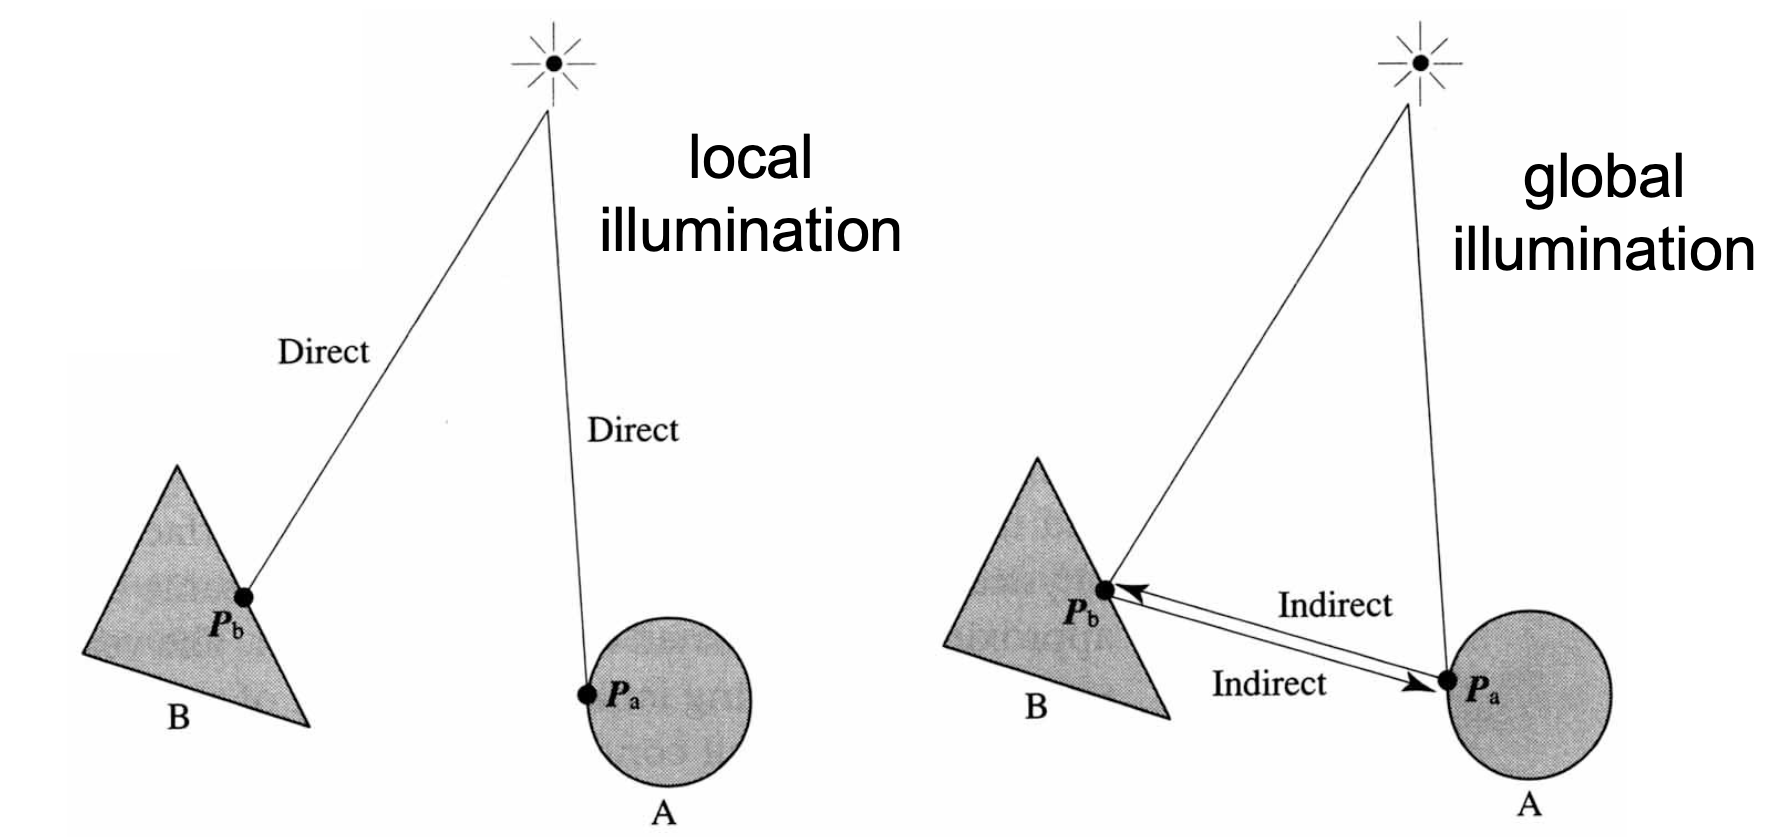
\includegraphics[width=\columnwidth]{L7/local_global}
    \end{center}
\section*{\normalsize Phong Illumination Eqn}
  \noindent
  \large
  \begin{align*}
    I_{Phong} =& \; I_a k_a + f_{att} I_p k_d (N \cdot L) \\
               &+ f_{att} I_p k_s (R \cdot V)^n
  \end{align*}
  \small
  \begin{itemize}[leftmargin=*]
    \item Assumes $N, L, R, V$ are unit vectors
    \item Assume that light source is a point
  \end{itemize}
  \begin{center}
    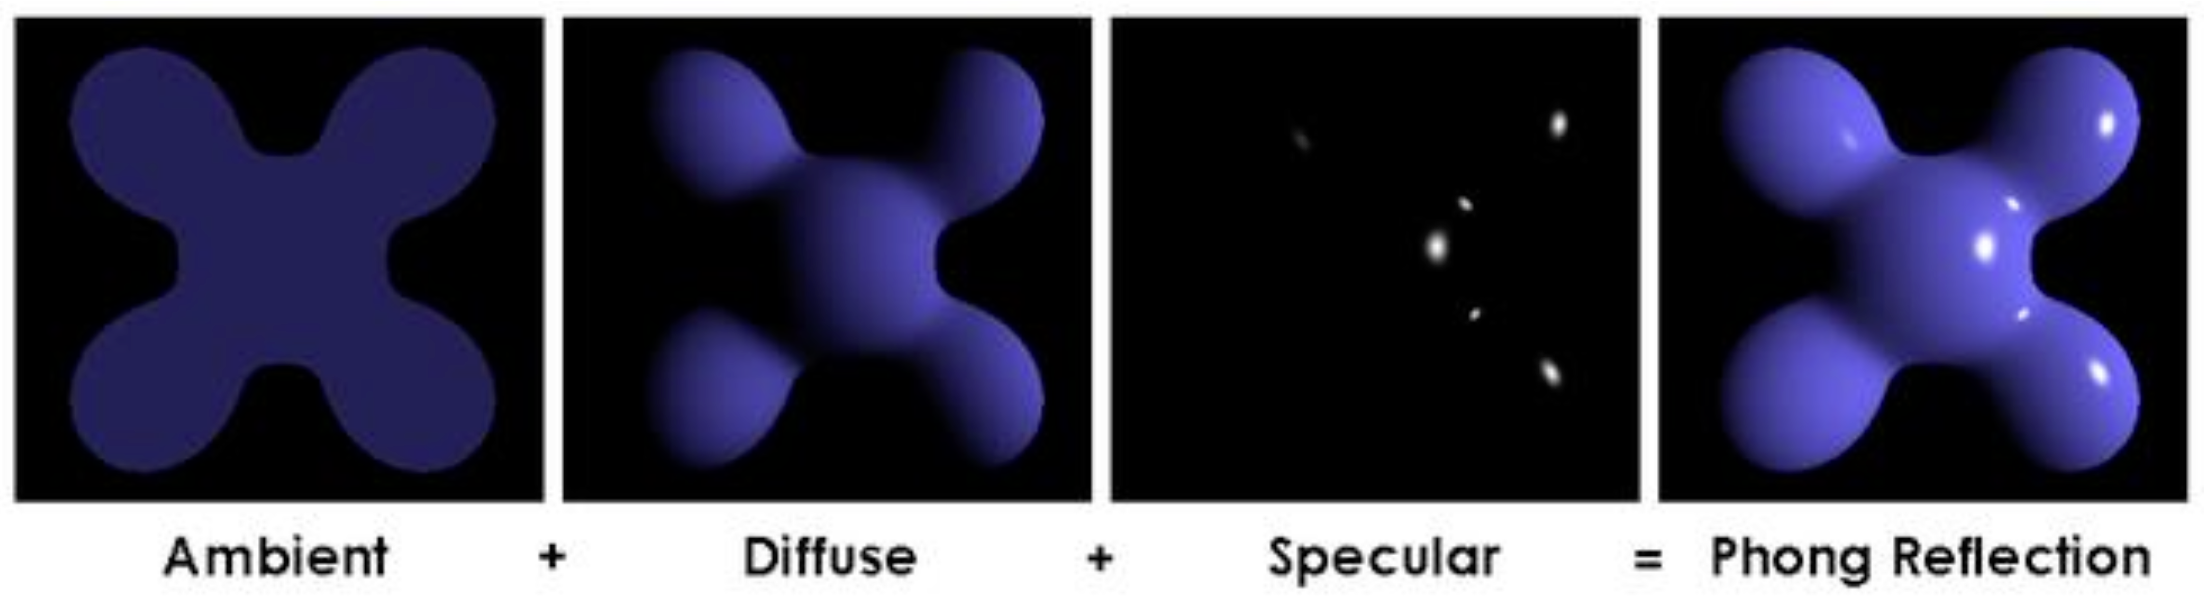
\includegraphics[width=\columnwidth]{L7/pie}
  \end{center}
  \subsection*{Ambient $I_a k_a$}
    \begin{itemize}[leftmargin=*]
      \item Produces a \uline{uniform} lighting effect (color, intensity) on every point on every surface
      \item Each surface has its own ambient material, so it can appear as a different color
    \end{itemize}
    \subsubsection*{Math}
      \begin{itemize}[leftmargin=*]
        \item $I_a$ is the luminance of the light
        \item $k_a$ is the ambient material property
      \end{itemize}
  \subsection*{Diffuse $f_{att} I_p k_d (N \cdot L)$}
    \begin{itemize}[leftmargin=*]
      \item Gives color to the surface point according to \uline{light position} and \uline{surface normal}
    \end{itemize}
    \subsubsection*{Surface normal}
      \begin{itemize}[leftmargin=*]
        \item Triangle with vertices $A,B,C$: $N = \pm (B-A) \times (C-A)$, consider the sign appropriately using RHGR
        \item Curved surface: normal of the plane tangent to that point
      \end{itemize}
    \subsubsection*{Lambert's cosine law}
      \begin{center}
        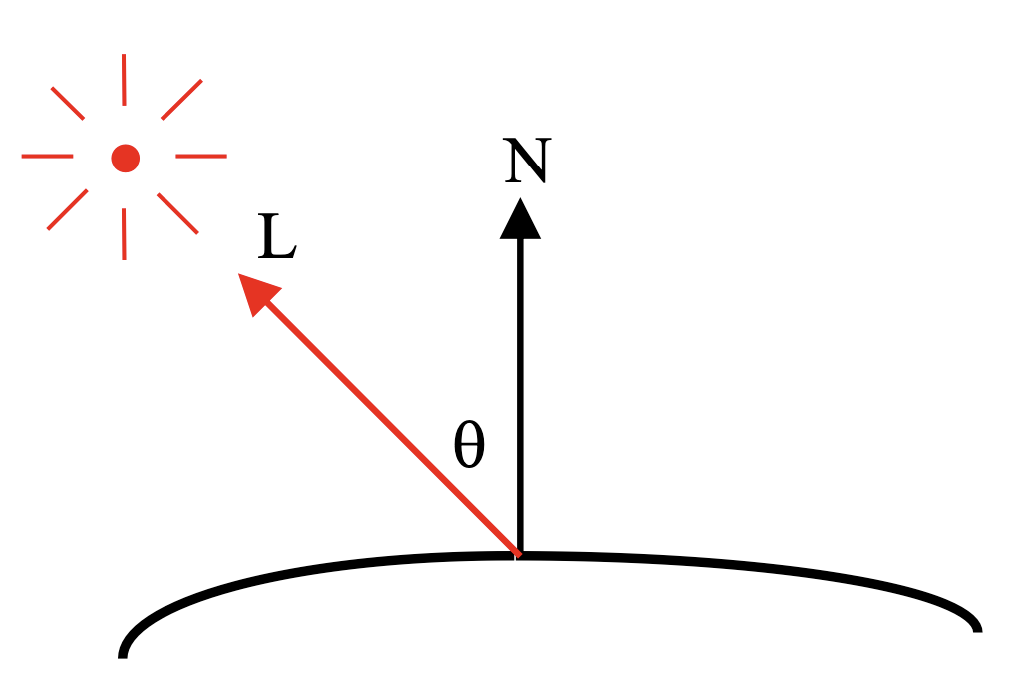
\includegraphics[width=0.7\columnwidth]{L7/diffuse}
      \end{center}
      States that diffuse reflection $\propto \cos \theta = N \cdot L$
    \subsubsection*{Attenuation factor $f_{att}$}
      \begin{itemize}[leftmargin=*]
        \item As the distance $d$ from the point to the light source increases, the light received will be weaker
        \item In physics, it is $\propto \dfrac{1}{d^2}$. If $d$ changes slightly, the light intensity can change significantly
        \item In OpenGL, we use $f_{att} = \dfrac{1}{a + bd + cd^2}$ to allow more granular control
      \end{itemize}
    \subsubsection*{Math}
      \begin{itemize}[leftmargin=*]
        \item $I_p$ is the luminance of the light coming from a point $p$
        \item $k_d$ is the diffuse material property
        \item $N \cdot L$ is for diffuse reflection
        \item $f_{att} = \dfrac{1}{a + bd + cd^2}$ is the attenuation factor, for some user-defined constants $a, b, c$
      \end{itemize}
  \subsection*{Specular $f_{att} I_p k_s (R \cdot V)^n$}
    \begin{itemize}[leftmargin=*]
      \item Adds highlights to shiny surface
    \end{itemize}
    \subsubsection*{Highlight}
      \begin{itemize}[leftmargin=*]
        \item Because we assume that the light source is a point, shininess is inversely propotional to the size of the highlight
        \item Highlight is dependent on $V$, because the highlight moves when the viewer moves
      \end{itemize}
    \begin{center}
      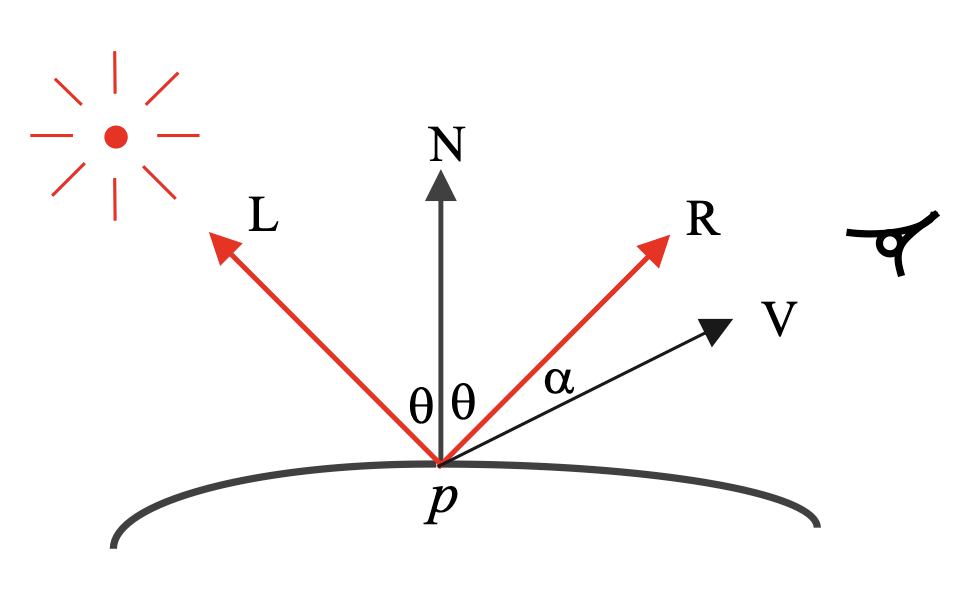
\includegraphics[width=0.8\columnwidth]{L7/specular}
    \end{center}
    \subsubsection*{Math}
      \begin{itemize}[leftmargin=*]
        \item Assume $N, L, R, V$ are unit vectors
          \begin{align*}
            \alpha &= \cos^{-1} (R \cdot V) \\
            R &= 2 (N \cdot L) N - L
          \end{align*}
        \item $k_s$ is the specular material property
        \item $n$ is the shininess coefficient - as $n$ increases, highlights become smaller and sharper
        \item $I_p$ and $f_{att}$ are defined in the diffuse section
      \end{itemize}
  \subsection*{Material properties}
    \begin{itemize}[leftmargin=*]
      \item Modelled using $k_a, k_d, k_s$ and $n$
      \item $k_a, k_d, k_s$ are vectors of 3 RGB colors, taking values between 0 and 1
      \item Shininess coefficient $n$ has value from 1 to 128 in OpenGL
    \end{itemize}
  \subsection*{Multiple light sources}
    \noindent
    \begin{gather*}
      I_{Phong} = \; I_a k_a + \\
      \sum_i f_{att} I_p k_d (N \cdot L_i) + f_{att} I_p k_s (R_i \cdot V)^n
    \end{gather*}
  \subsection*{Blinn-Phong model (T6)}
    \begin{align*}
      I_{Blinn-Phong} =& \; I_a k_a + I_p k_d (N \cdot L) \\
                       &+ I_p k_s (N \cdot H)^n
    \end{align*}
    where $H = \mathrm{normalize}(L + V)$
    \begin{itemize}[leftmargin=*]
      \item Produces larger specular highlights than Phong model
      \item More efficient if light source and viewer are far apart, because $L$ and $V$ will be roughly the same for all the surface points, so $H$ also does not need to be recomputed
    \end{itemize}
  \subsection*{Retroreflection (T6)}
    \begin{itemize}[leftmargin=*]
      \item A retroreflector reflects most of the light back in the incident direction
      \item Set $R=L$ in Phong equation
      \item e.g. Cat's eye, road signs
    \end{itemize}
\section*{\normalsize Illumination in OpenGL}
  \begin{itemize}[leftmargin=*]
    \item Vertex processing stage: model-view transformation, \uline{lighting computation}, texture coordinates, then projection to clip space
    \item Since it is between the model view transformation and the projection matrix, it is performed in \uline{eye/camera space}
  \end{itemize}
  \subsubsection*{Specify vertex normal}
    \begin{itemize}[leftmargin=*]
      \item Use \ic{glNormal3f(x, y, z)} or \ic{glNormal3fv(p)}
      \item Normal should have unit length. Use \ic{glEnable(GL_NORMALIZE)} for auto-normalization, with a performance penalty
    \end{itemize}
  \subsubsection*{Enable lighting computation}
    \begin{itemize}[leftmargin=*]
      \item Use \ic{glEnable(GL_LIGHTING)}. Thereafter, \ic{glColor()} is ignored
      \item Use \ic{glEnable(GL_LIGHTi)} to enable light source $i$, where $0 \leq i \leq 7$ (OpenGL supports 8 lights)
      \item Use \ic{glLightModeli(param, GL_TRUE)} to activate certain light model parameters
        \begin{itemize}[leftmargin=*]
          \item \ic{GL_LIGHT_MODEL_LOCAL_VIEWER} sets the view ray to be from each surface point to the origin of the eye coordinate system, for computing specular reflections. Otherwise, it is taken to be parallel to and in the direction of the $-z$ axis.
          \item \ic{GL_LIGHT_MODEL_TWO_SIDED} shades both sides of polygons independently
        \end{itemize}
    \end{itemize}
  \subsubsection*{Defining a point light source}
    \begin{lstlisting}
// RGBA values
GLfloat a0[] = {1.0, 0.0, 0.0, 1.0};
GLfloat d0[] = {1.0, 0.0, 0.0, 1.0};
GLfloat s0[] = {1.0, 0.0, 0.0, 1.0};
GLfloat p0[] = {1.0, 2.0, 3.0, 1.0};

glEnable(GL_LIGHTING);
glEnable(GL_LIGHT0);
glLightfv(GL_LIGHT0, GL_POSITION, p0);
glLightfv(GL_LIGHT0, GL_AMBIENT, a0);
glLightfv(GL_LIGHT0, GL_DIFFUSE, d0);
glLightfv(GL_LIGHT0, GL_SPECULAR, s0);
    \end{lstlisting}
  \subsubsection*{Enable global ambient light}
    \begin{itemize}[leftmargin=*]
      \item \ic{glLightModelfv(GL_LIGHT_MODEL_AMBIENT, global_ambient)}
    \end{itemize}
  \subsubsection*{Moving light sources}
    \begin{itemize}[leftmargin=*]
      \item The positions and directions of light sources are affected by the model-view transformation
    \end{itemize}
  \subsubsection*{Setting material properties}
    \begin{lstlisting}
// RGBA values
GLfloat a[] = {0.2, 0.2, 0.2, 1.0};
GLfloat d[] = {1.0, 0.8, 0.0, 1.0};
GLfloat s[] = {1.0, 1.0, 1.0, 1.0};
GLfloat shine = 100.0;

glMaterialfv(GL_FRONT, GL_AMBIENT, a);
glMaterialfv(GL_FRONT, GL_DIFFUSE, d);
glMaterialfv(GL_FRONT, GL_SPECULAR, s);
glMaterialfv(GL_FRONT, GL_SHININESS, shine);
    \end{lstlisting}
  \subsubsection*{Customizing front/back faces}
    \begin{itemize}[leftmargin=*]
      \item Default behaviour shades only front faces, which works correctly for convex objects
      \item If set two sided lighting (see Enable lighting computation), OpenGL shades both sides of a surface
      \item Use \ic{GL_FRONT}, \ic{GL_BACK}, \ic{GL_FRONT_AND_BACK} to set properties of each side
    \end{itemize}
  \subsubsection*{Emissive term}
    \begin{itemize}[leftmargin=*]
      \item Can simulate a light source by giving a material an emissive component
      \item Not affected by any sources or transformations
    \end{itemize}
    \begin{lstlisting}
GLfloat e[] = {0.0, 0.3, 0.3, 1.0};
glMaterialfv(GL_FRONT, GL_EMISSION, emission);
    \end{lstlisting}
  \subsection*{OpenGL lighting comp formula}
    \begin{center}
      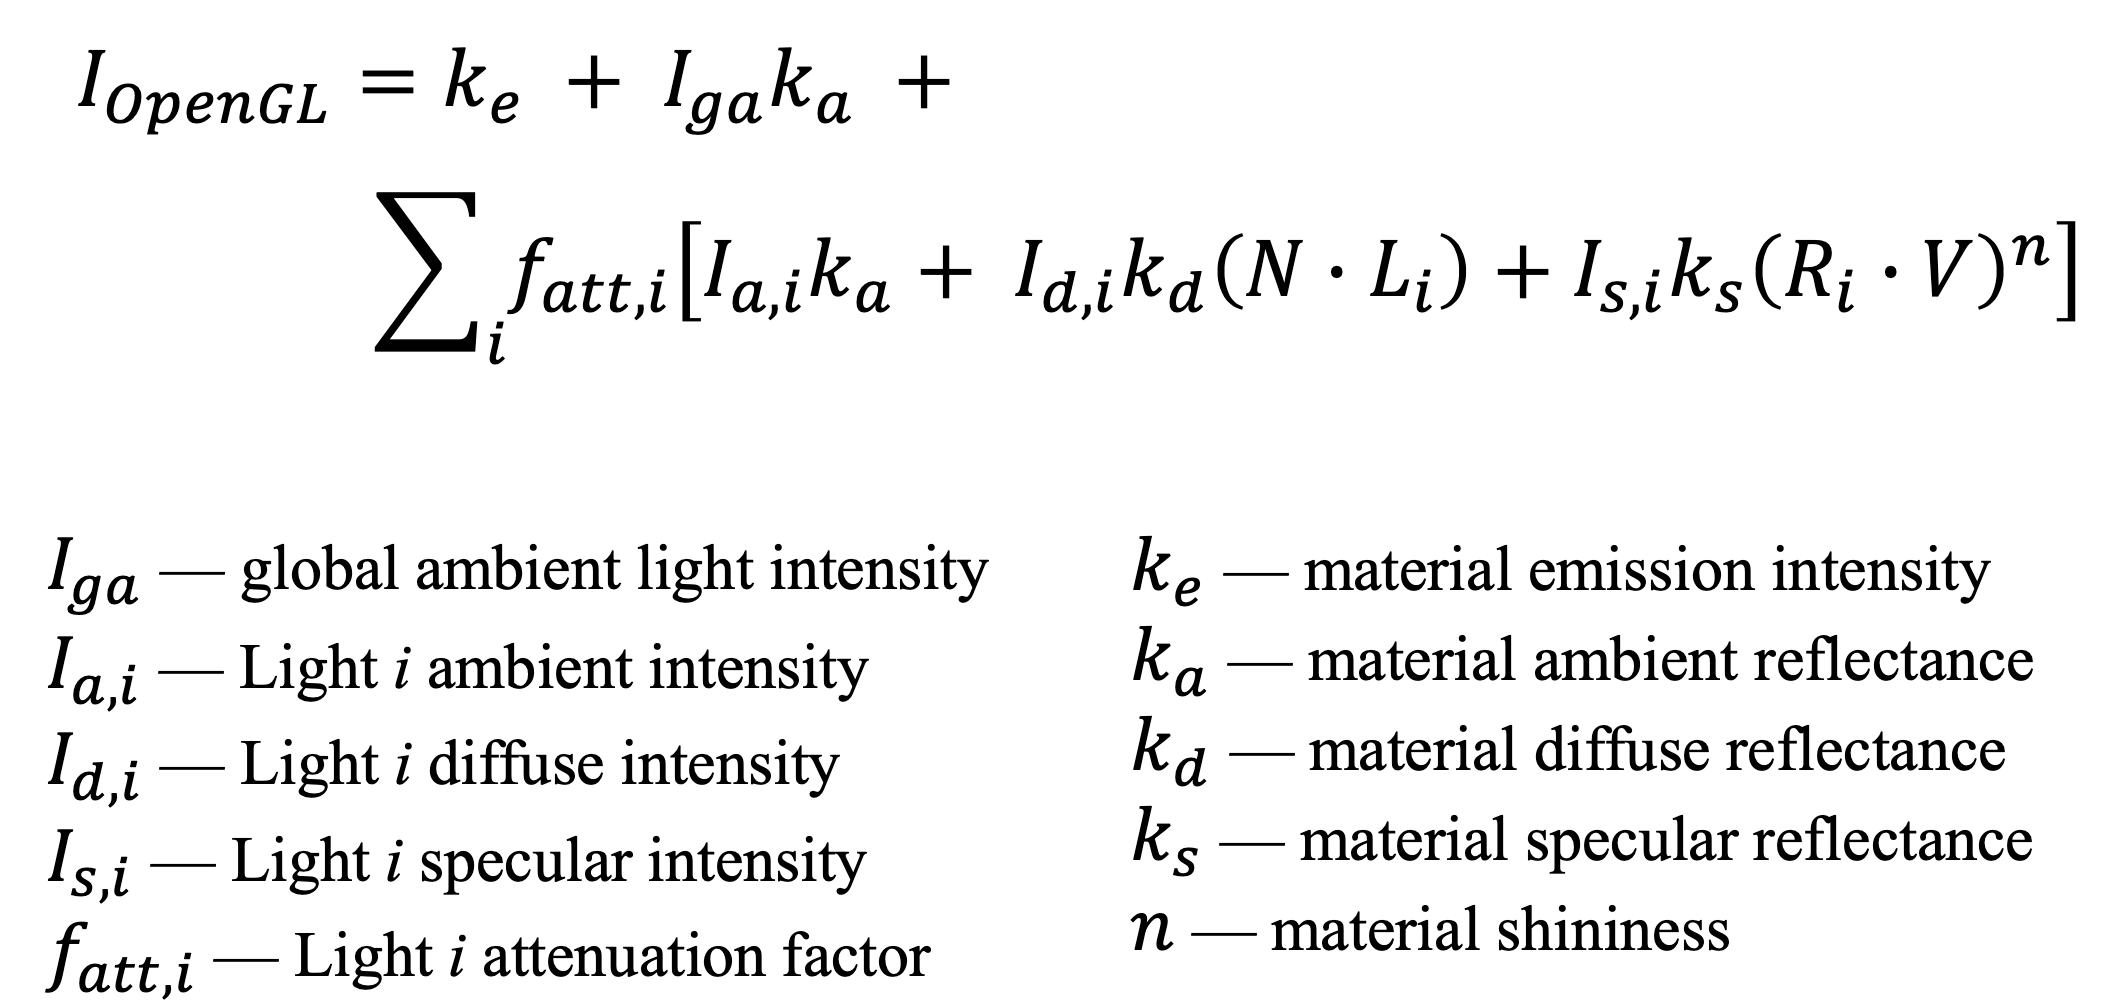
\includegraphics[width=\columnwidth]{L7/opengl_formula}
    \end{center}
\section*{\normalsize Shading}
  \begin{center}
    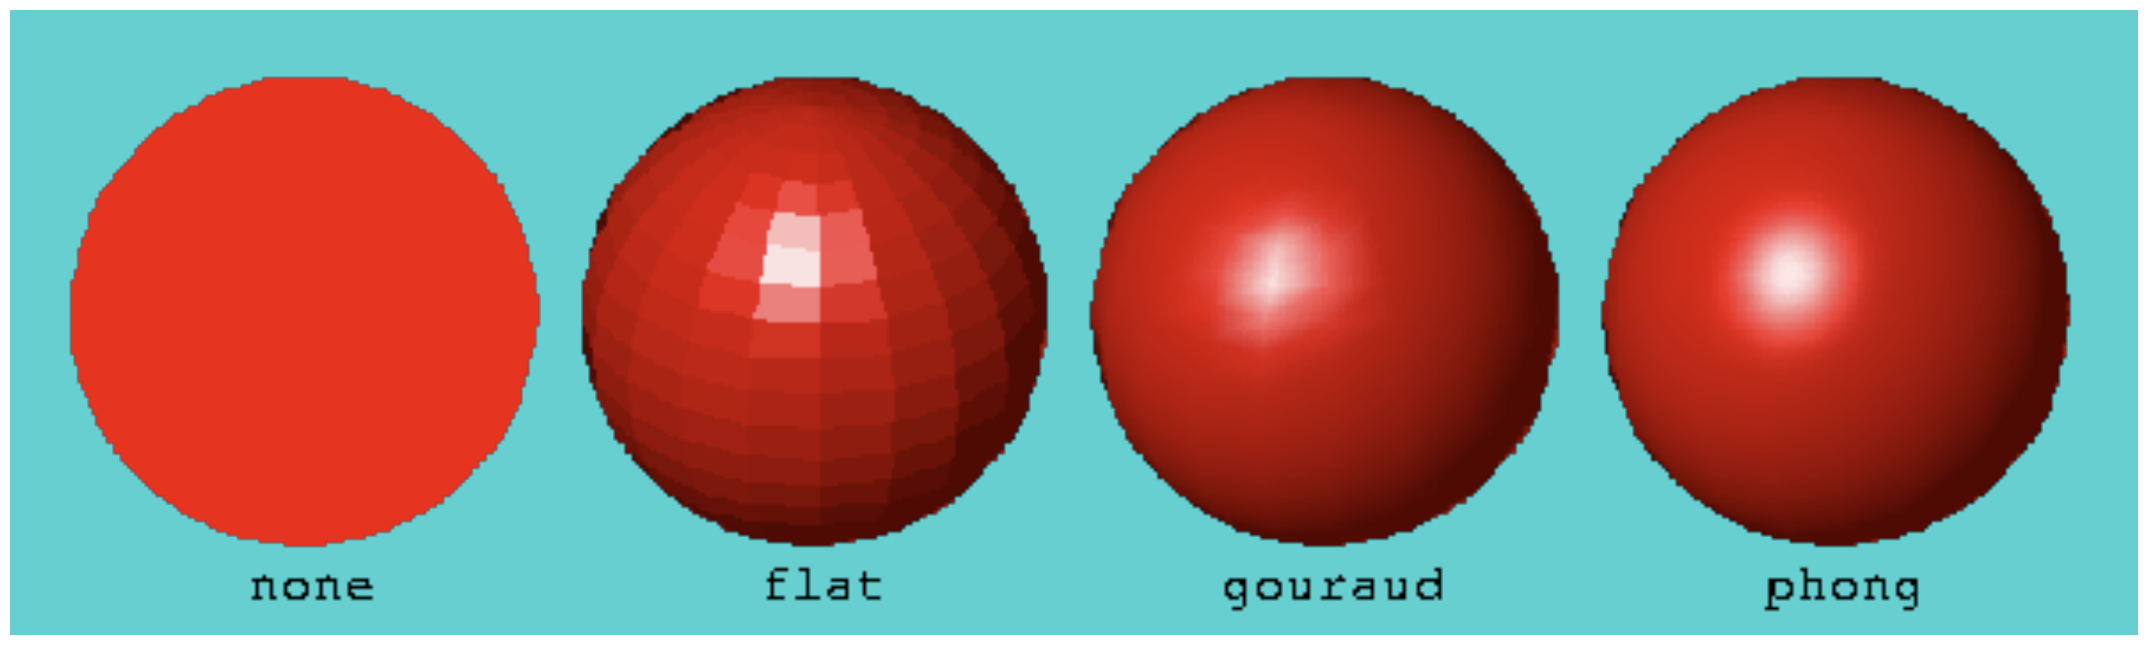
\includegraphics[width=\columnwidth]{L7/shading}
  \end{center}
  \subsection*{Flat shading}
    \begin{itemize}[leftmargin=*]
      \item Choose any vertex of the polygon, compute its color with PIE, apply that color to the polygon
      \item Each polygon has one color
      \item Distinctive color difference between neighbouring polygons
      \item \ic{glShadeModel(GL_FLAT)}
    \end{itemize}
  \subsection*{Gouraud shading}
    \begin{center}
      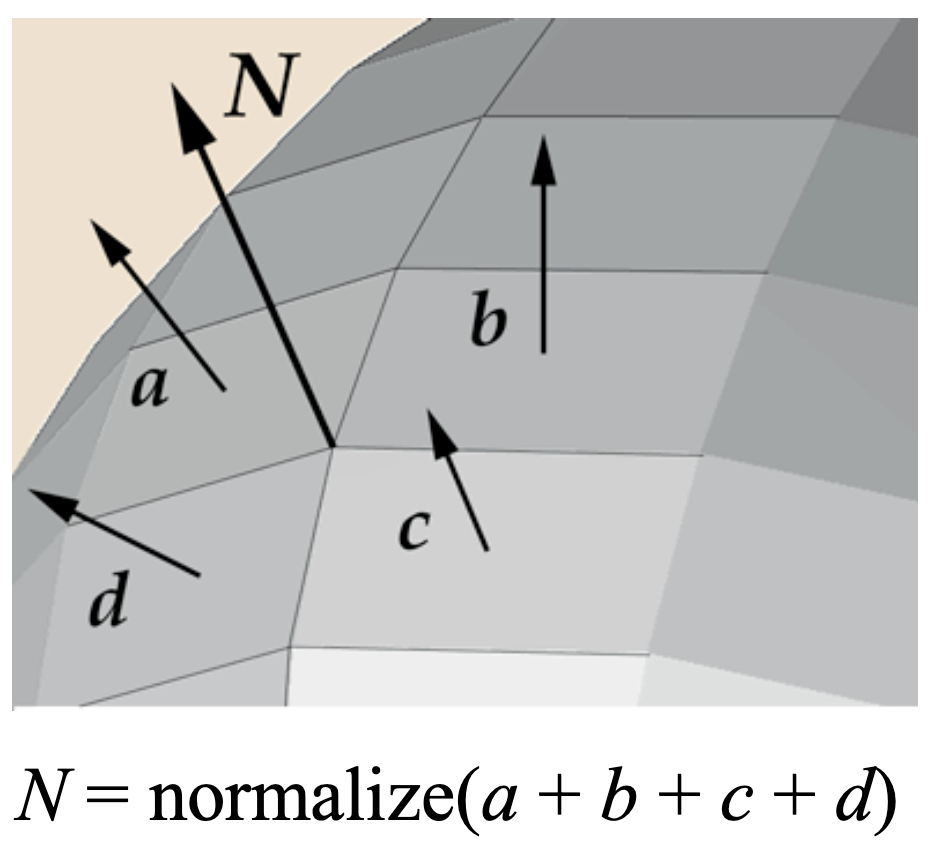
\includegraphics[width=0.7\columnwidth]{L7/gouraud}
    \end{center}
    \begin{itemize}[leftmargin=*]
      \item For each vertex, compute the average normal vector of polygons sharing that vertex (so we need to know how to find neighbouring polygons)
      \item Apply PIE at the vertex using the average normal vector
      \item Smoothly interpolate computed colors at vertices of the polygon to the interior of the polygon
      \item Per-vertex lighting computation
      \item \ic{glShadeModel(GL_SMOOTH)}
    \end{itemize}
  \subsection*{Phong shading}
    \begin{itemize}[leftmargin=*]
      \item For each fragment in the polygon, interpolate normal vectors from vertices
      \item Apply PIE at the fragment using the interpolated normal vector
      \item Per-fragment (pixel) lighting computation, hence generally more expensive than Gouraud shading
      \item Better at producing highlights, since each fragment has its own normal vector
      \item Not supported by OpenGL, but can be supported by reprogramming the rendering pipeline using shaders
    \end{itemize}
\section*{Texture Mapping}
  \subsection*{Overview}
    \begin{center}
      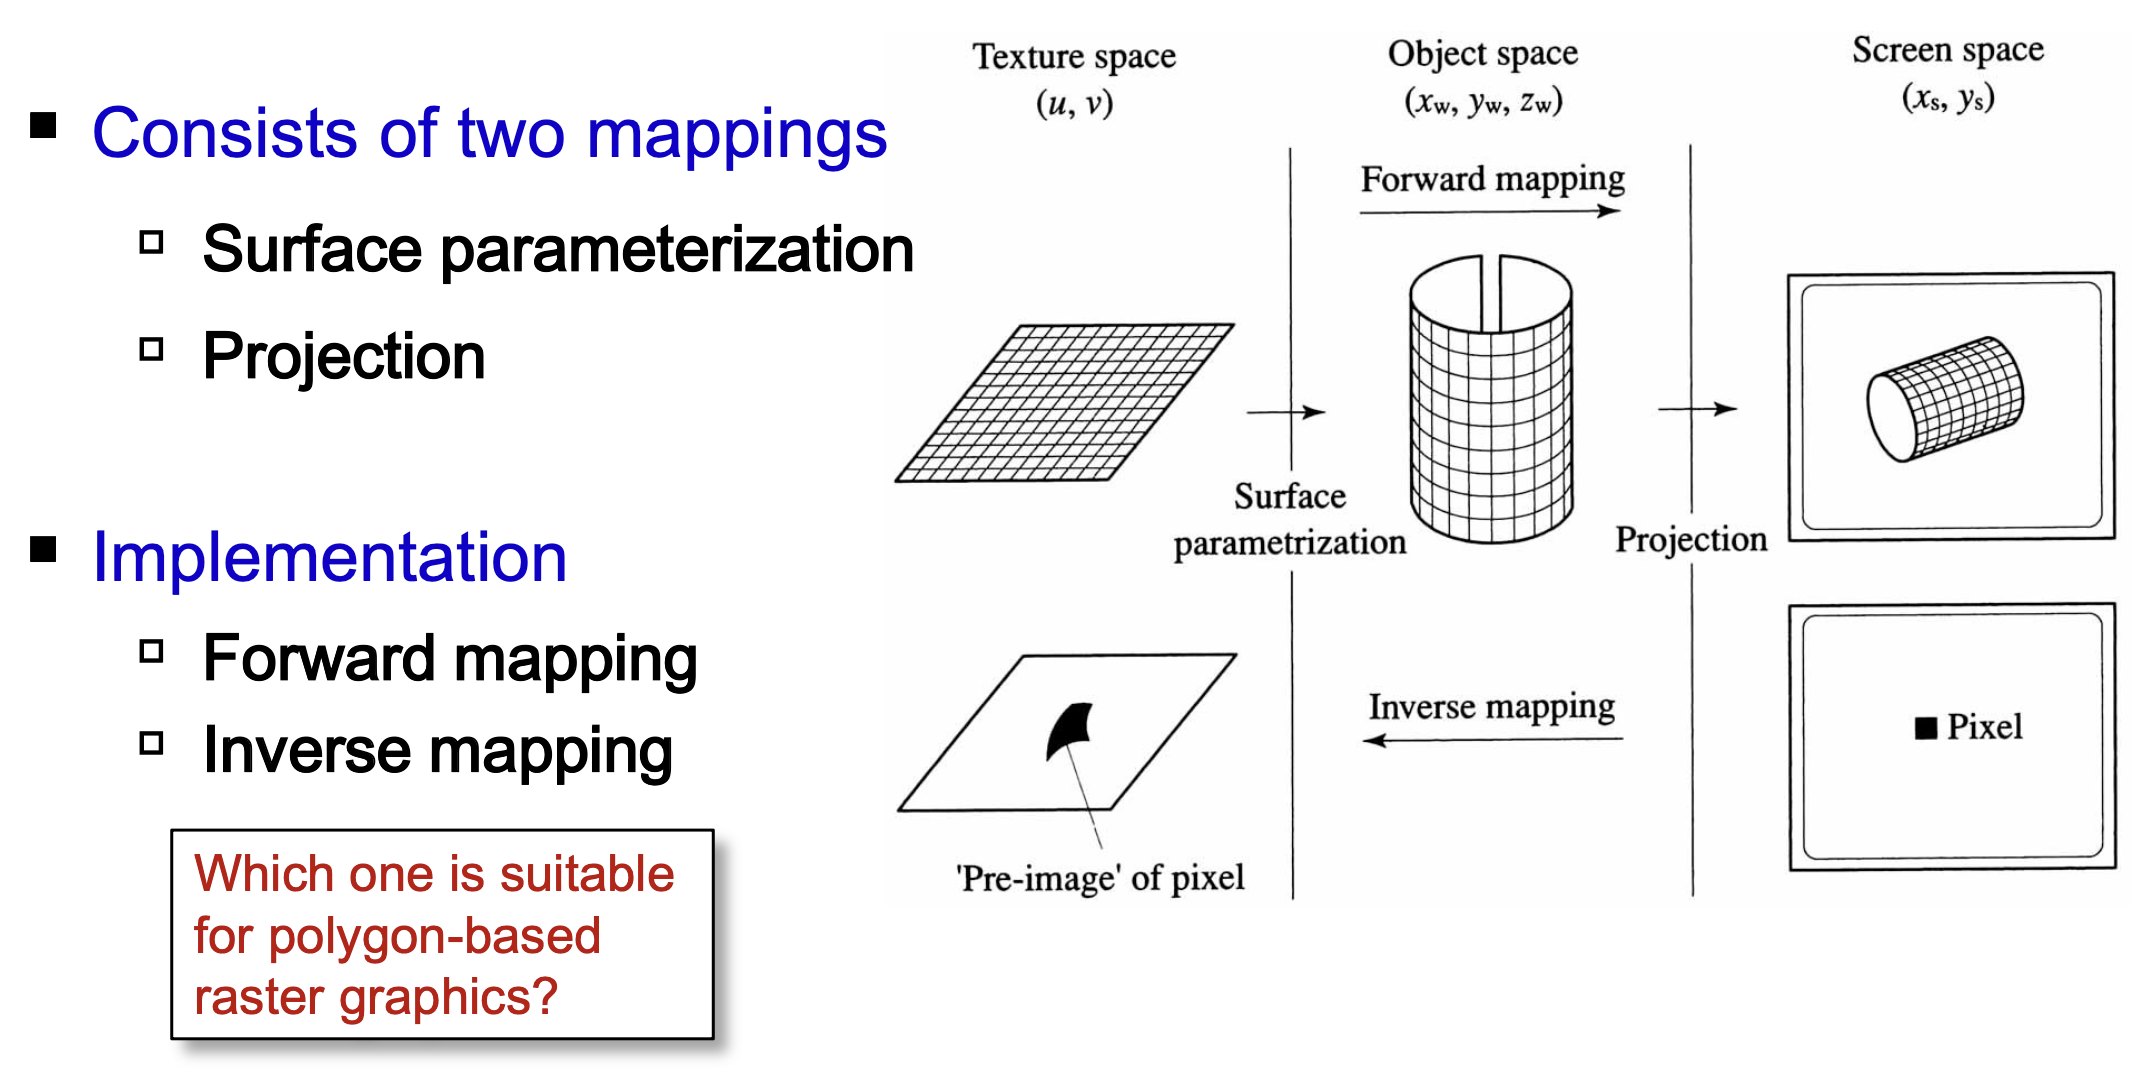
\includegraphics[width=\columnwidth]{L8/overview}
    \end{center}
    \begin{itemize}[leftmargin=*]
      \item Forward mapping only guarantees that each texel maps to some point in the screen space. Each pixel in screen space may have 0, 1, or many texels mapped to it, which is not ideal.
      \item Inverse mapping guarantees that each pixel has exactly 1 texel mapped to it.
    \end{itemize}
  \subsection*{Surface parameterization}
    \begin{itemize}[leftmargin=*]
      \item Defines a mapping between 3D surface and 2D texture map
      \item $(x_w, y_w, z_w) \leftrightarrow (s, t)$, where $0 \leq s, t \leq 1$
      \item For polygonal models, texture coordinates are specified at vertices, and interpolated over the polygon
      \item Non-trivial surface topology can cause severe distortion of textures
    \end{itemize}
    \subsubsection*{How to parameterize}
      \begin{center}
        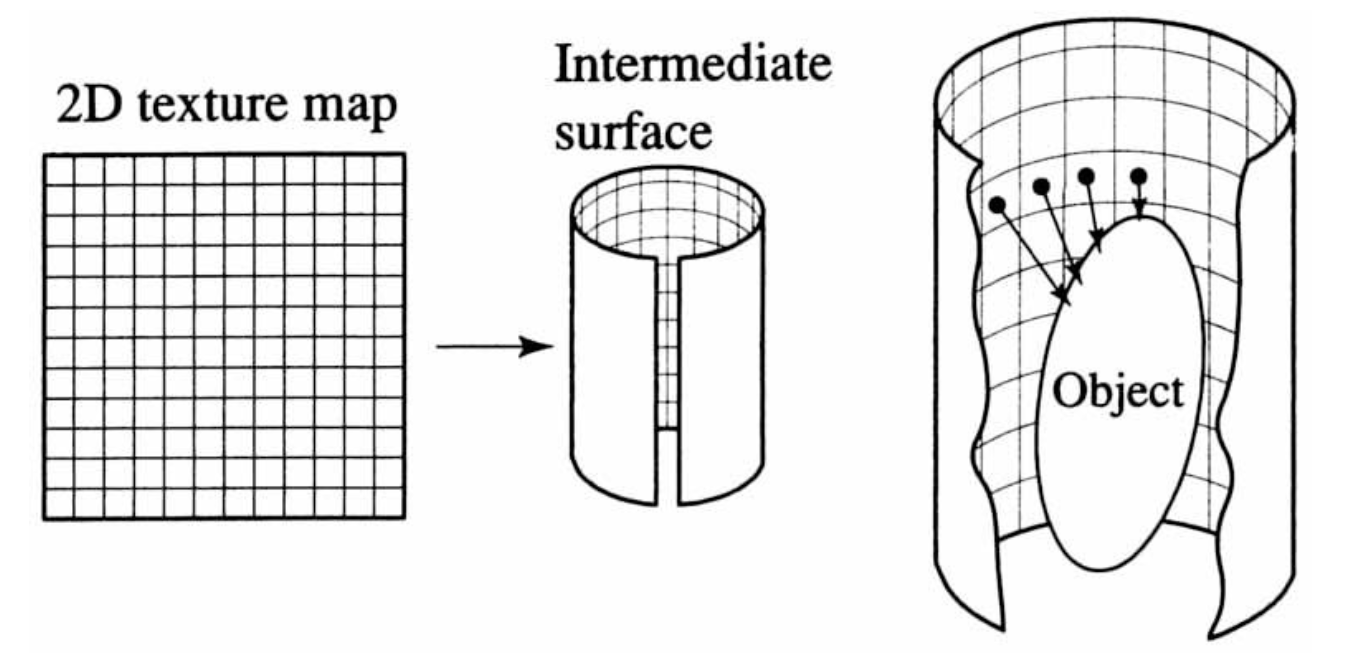
\includegraphics[width=\columnwidth]{L8/parameterization}
      \end{center}
      \begin{itemize}[leftmargin=*]
        \item First, apply S mapping - Texture map is projected onto a simple intermediate surface (e.g. plane, cylinder, sphere, cube). Intermediate surface chosen should be the most representative of the object
        \item Then, apply O mapping - 3D intermediate surface is then mapped onto the object surface
      \end{itemize}
    \subsubsection*{O mapping methods}
      \begin{center}
        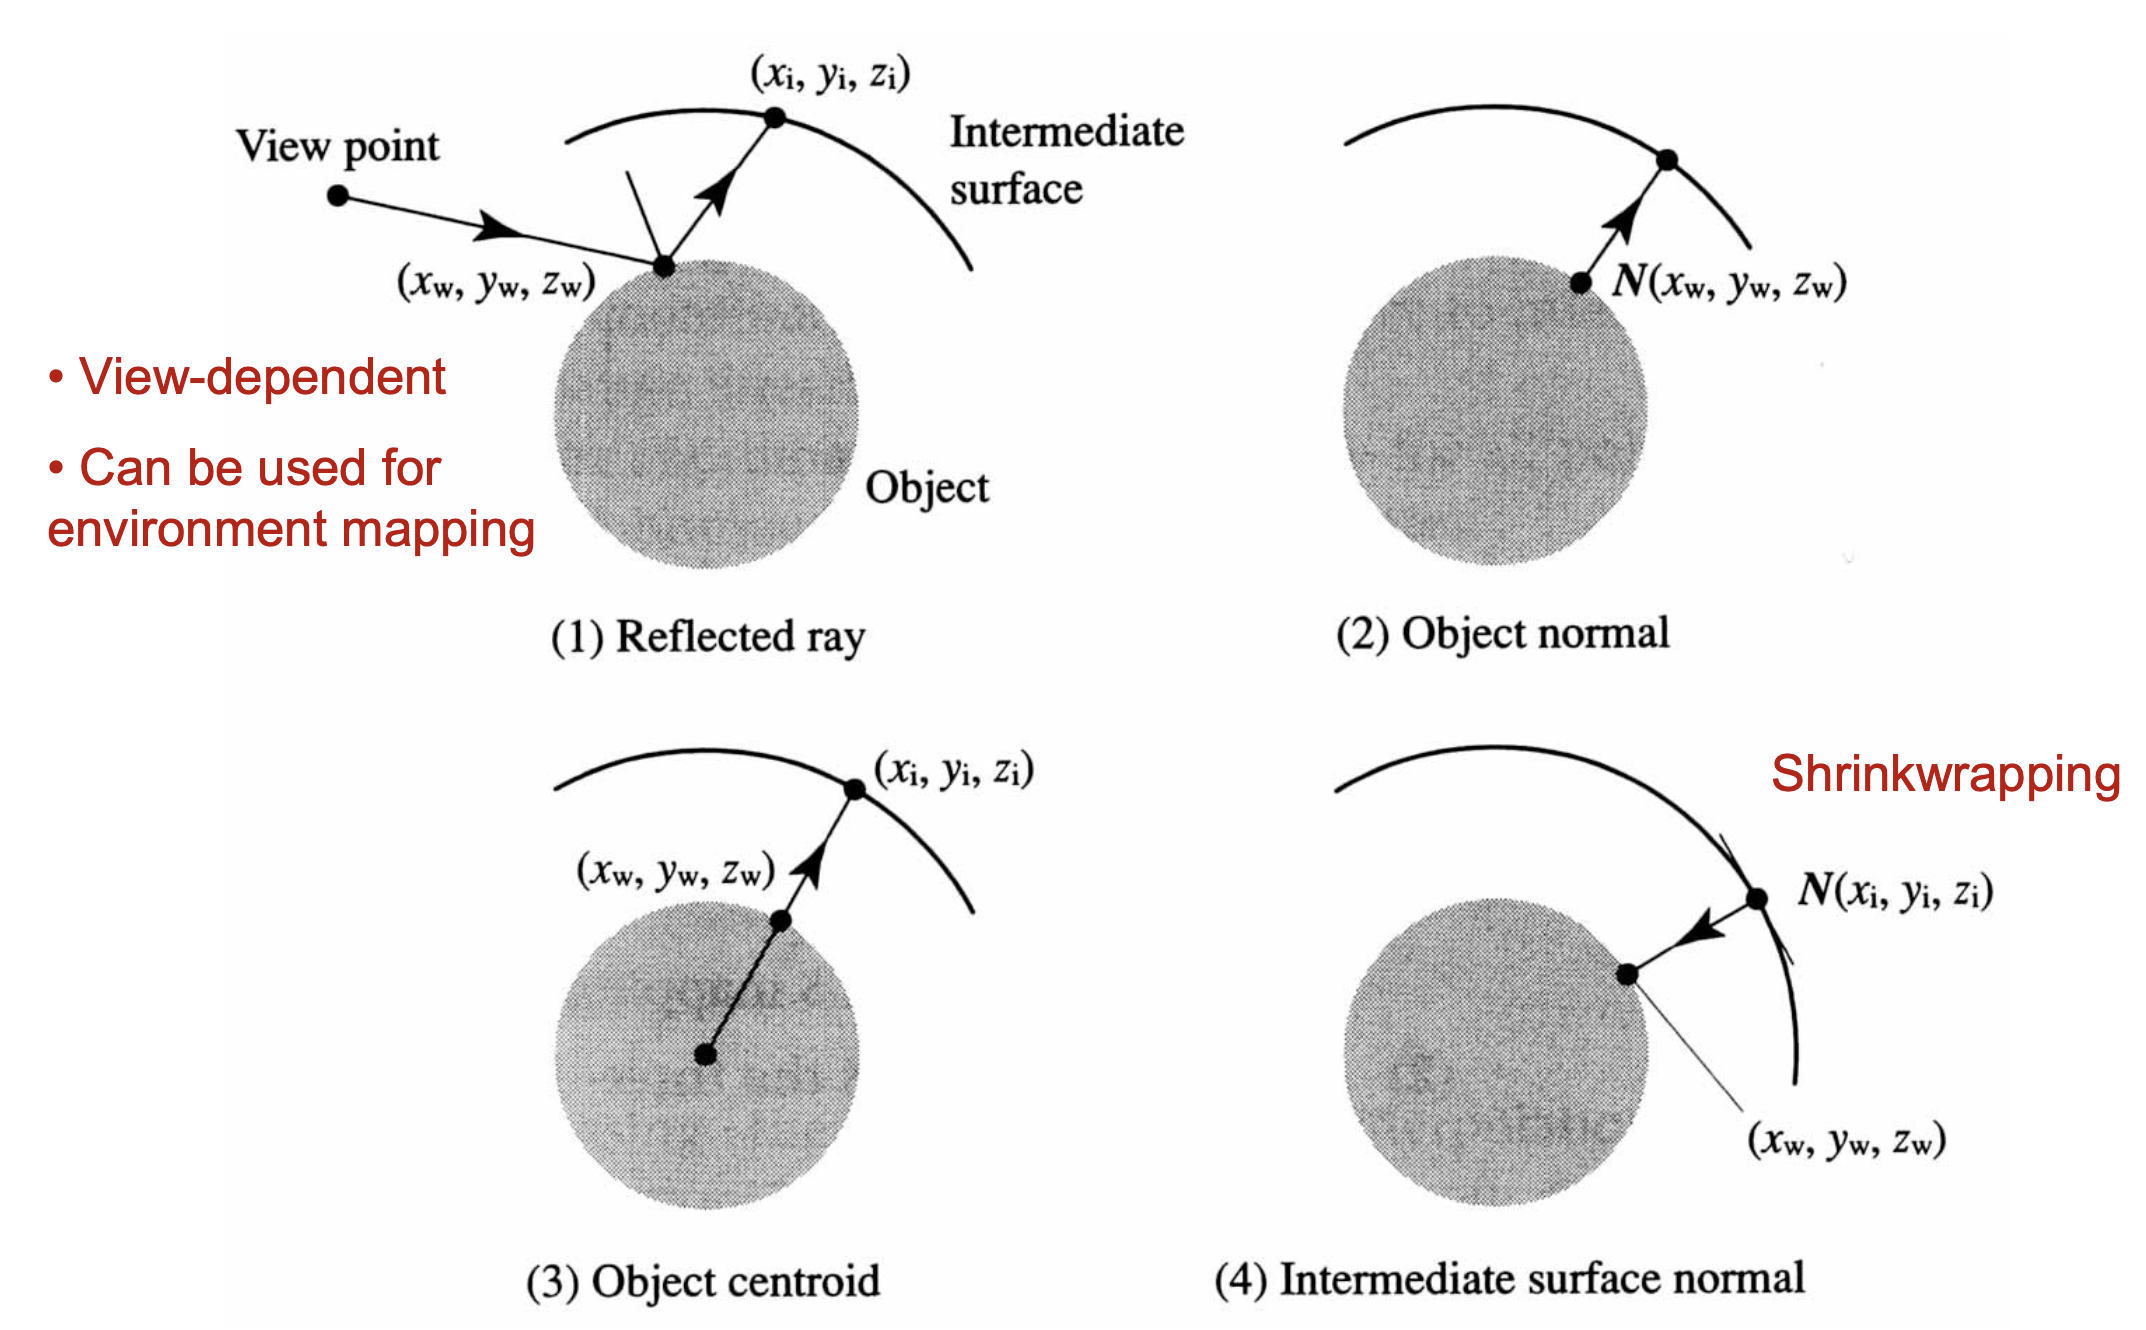
\includegraphics[width=\columnwidth]{L8/o_mapping}
      \end{center}
    \subsubsection*{Examples}
      \begin{center}
        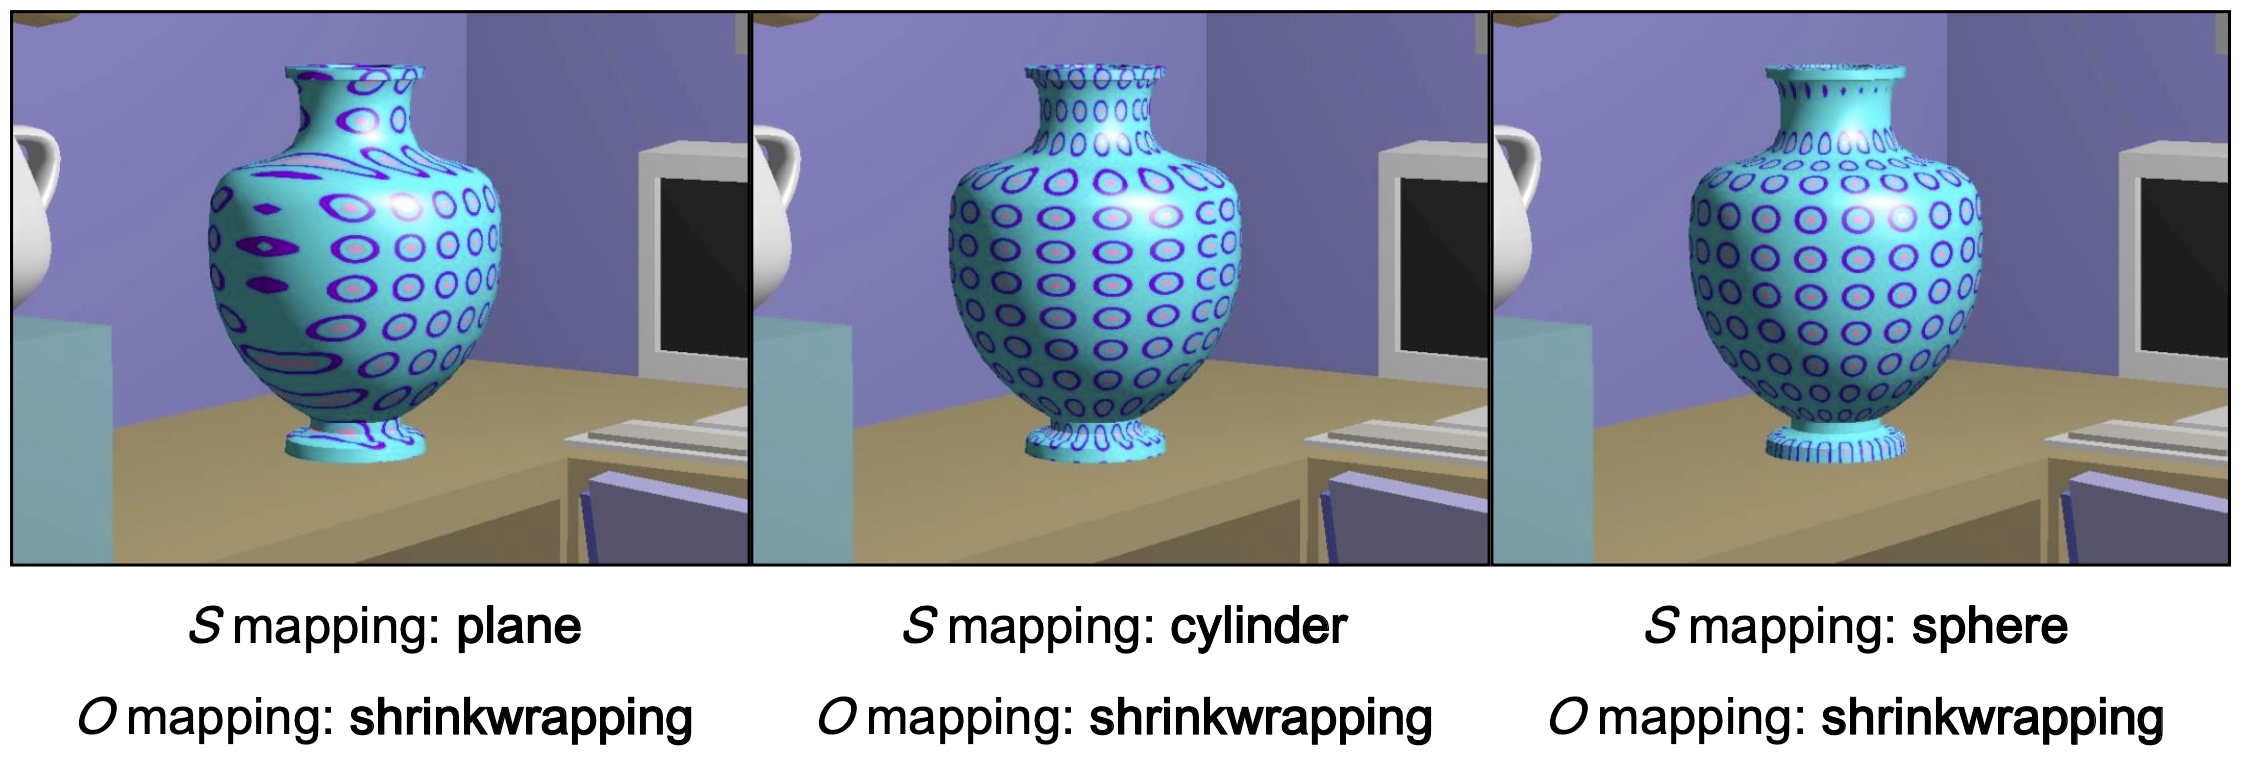
\includegraphics[width=\columnwidth]{L8/surface_parameterization_examples}
      \end{center}
  \subsection*{Texture coordinates mapping}
    \subsubsection*{Texture filtering}
      \begin{itemize}[leftmargin=*]
        \item At each fragment, the interpolated texture coordinates may not correspond to a texel center, so we need bilinear interpolation of adjacent texels
      \end{itemize}
      \begin{center}
        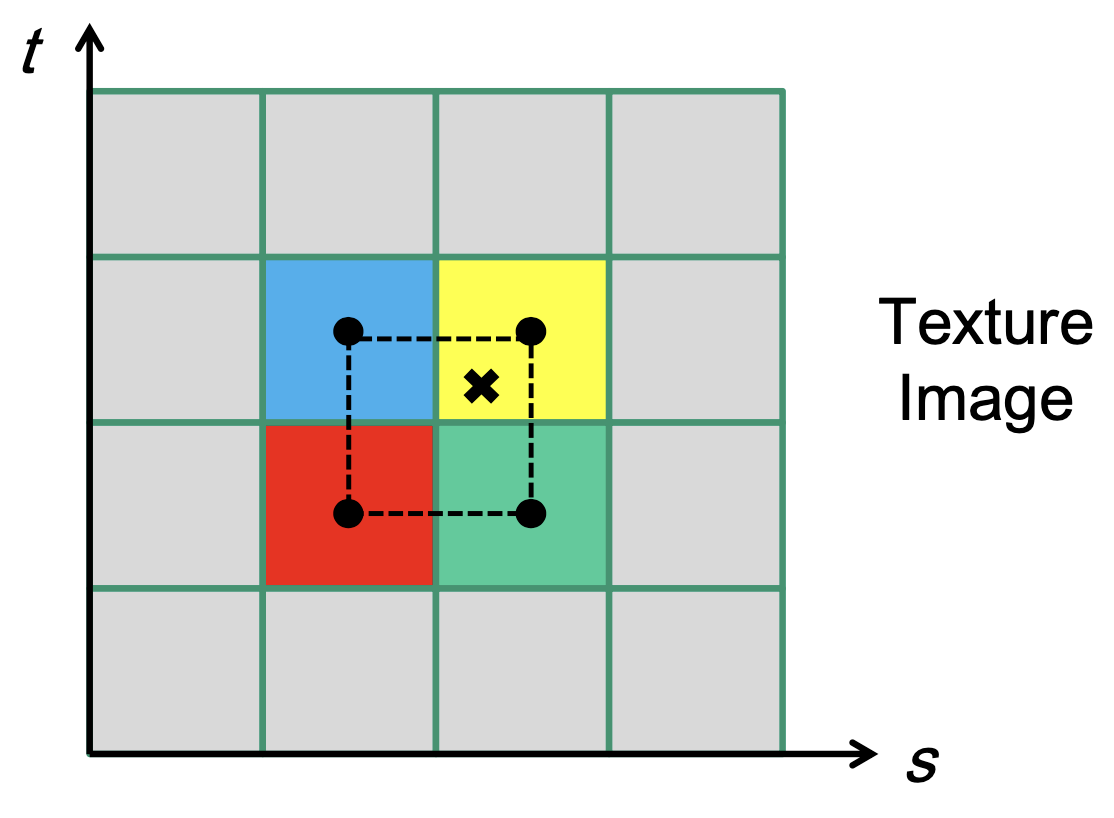
\includegraphics[width=\columnwidth]{L8/texture_filtering}
      \end{center}
    \subsubsection*{Wrapping}
      \begin{itemize}[leftmargin=*]
        \item Although we defined $0 \leq s,t \leq 1$, OpenGL allows vertex coordinates outside of this range
        \item Behaviour is defined according to the wrapping mode
          \begin{itemize}[leftmargin=*]
            \item Clamp \ic{GL_CLAMP_TO_EDGE} - clamped to $[0, 1]$
            \item Repeat \ic{GL_REPEAT} (default) - repeats the texture
          \end{itemize}
      \end{itemize}
      \begin{center}
        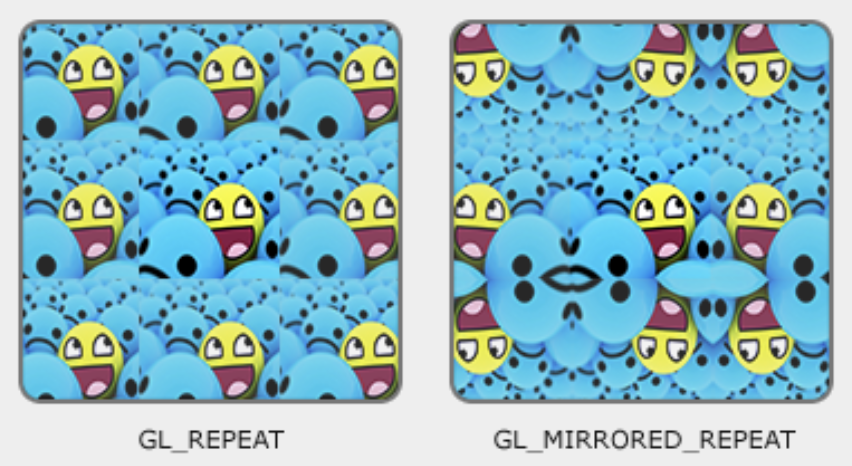
\includegraphics[width=0.7\columnwidth]{L8/texture_wrapping_1}
        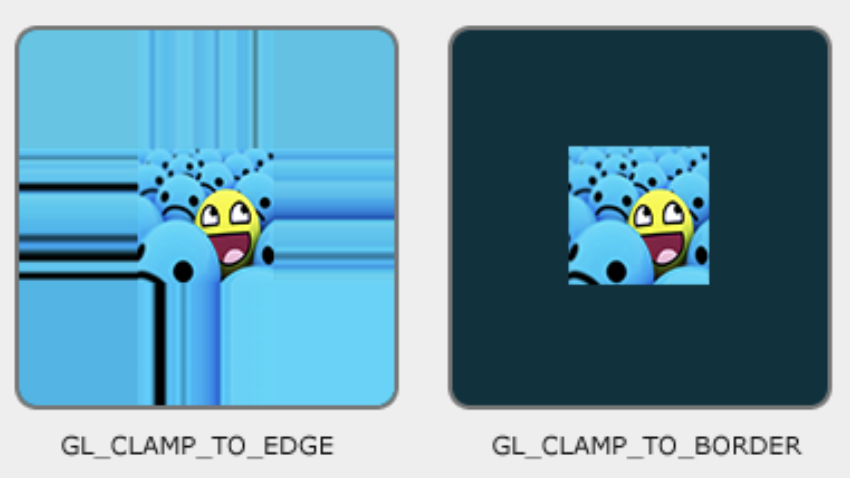
\includegraphics[width=0.7\columnwidth]{L8/texture_wrapping_2}
      \end{center}
  \subsection*{Anti-aliasing}
    \subsubsection*{Aliasing}
      \begin{itemize}[leftmargin=*]
        \item Aliasing can happen if texture map is point-sampled at each fragment
        \item Occurs during texture minification (when a big part of texture image is mapped to a single texel)
      \end{itemize}
    \subsubsection*{Anti-aliasing}
      \begin{itemize}[leftmargin=*]
        \item To fix, texture map should be area-sampled at each fragment
        \item A fragment is mapped to a quadrilateral area (pre-image) in the texture space, and the average color of the texels is used
      \end{itemize}
      \paragraph{Problems}
        \begin{itemize}[leftmargin=*]
          \item Need to find pre-image
          \item Need to sum the colors of several texels quickly
          \item Solution: mipmapping
        \end{itemize}
  \subsection*{Mipmapping}
    \begin{itemize}[leftmargin=*]
      \item Create a set of pre-filtered texture maps by approximating each pre-image using a square
      \item Point sample the appropriate texture map for each fragment according to the degree of texture minification
    \end{itemize}
    \subsubsection*{Creating mipmaps}
      \begin{center}
        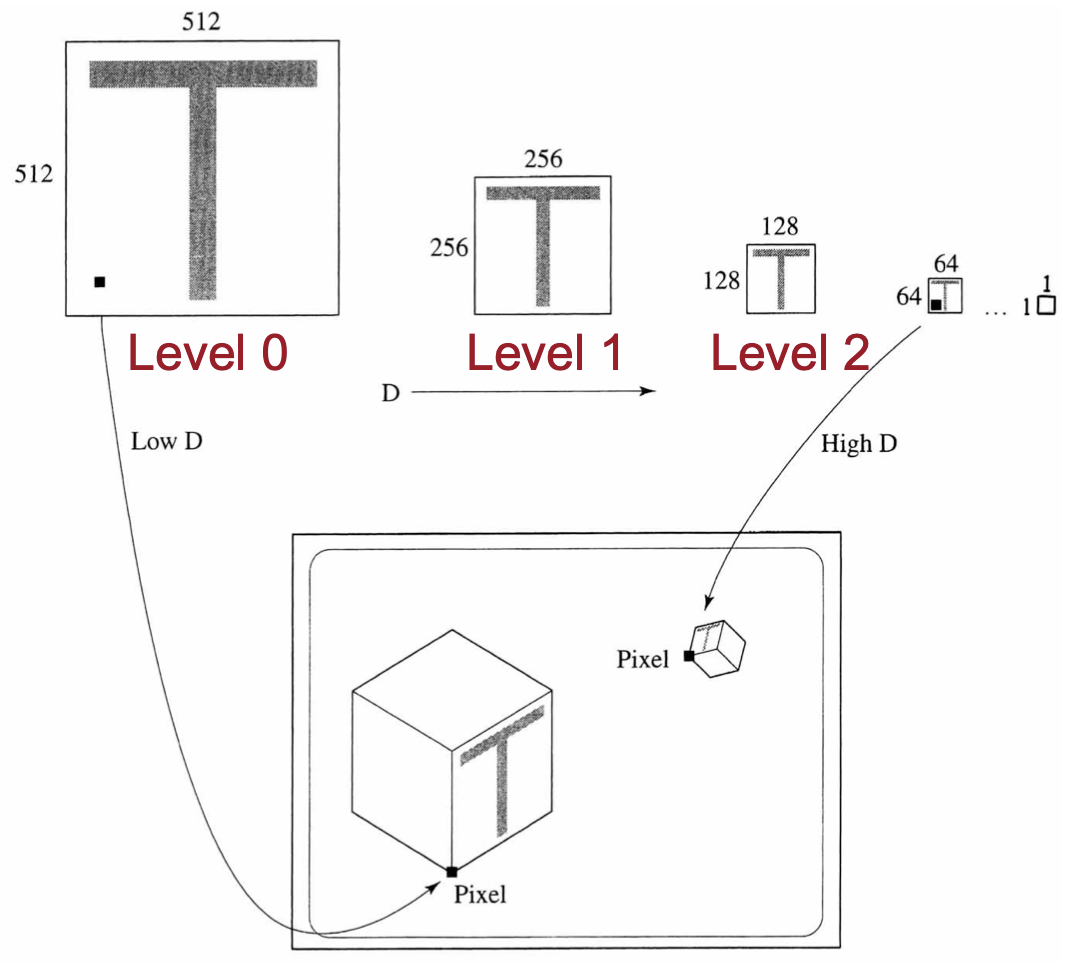
\includegraphics[width=\columnwidth]{L8/mipmapping}
      \end{center}
      \begin{itemize}[leftmargin=*]
        \item Created by averaging down the original image successively by half the resolution
        \item Starts at level 0 (original image)
        \item Each level halves the width and the height
      \end{itemize}
    \subsubsection*{Choosing mipmap level}
      \begin{itemize}[leftmargin=*]
        \item Choose according to amount of texture minification, e.g.
          \begin{itemize}[leftmargin=*]
            \item If fragment pre-image corresponds to $\leq 1$ texel, use mipmap level 0
            \item If fragment pre-image corresponds to $2 \times 2$ texels, use mipmap level 1
          \end{itemize}
        \item Ideal level may be non-integer
          \begin{itemize}[leftmargin=*]
            \item Perform linear interpolation of texels retrieved from two consecutive mipmap levels
            \item Called trilinear texture map interpolation
          \end{itemize}
      \end{itemize}
  \subsection*{Applications}
    \subsubsection*{Environment/Reflection mapping}
      \begin{center}
        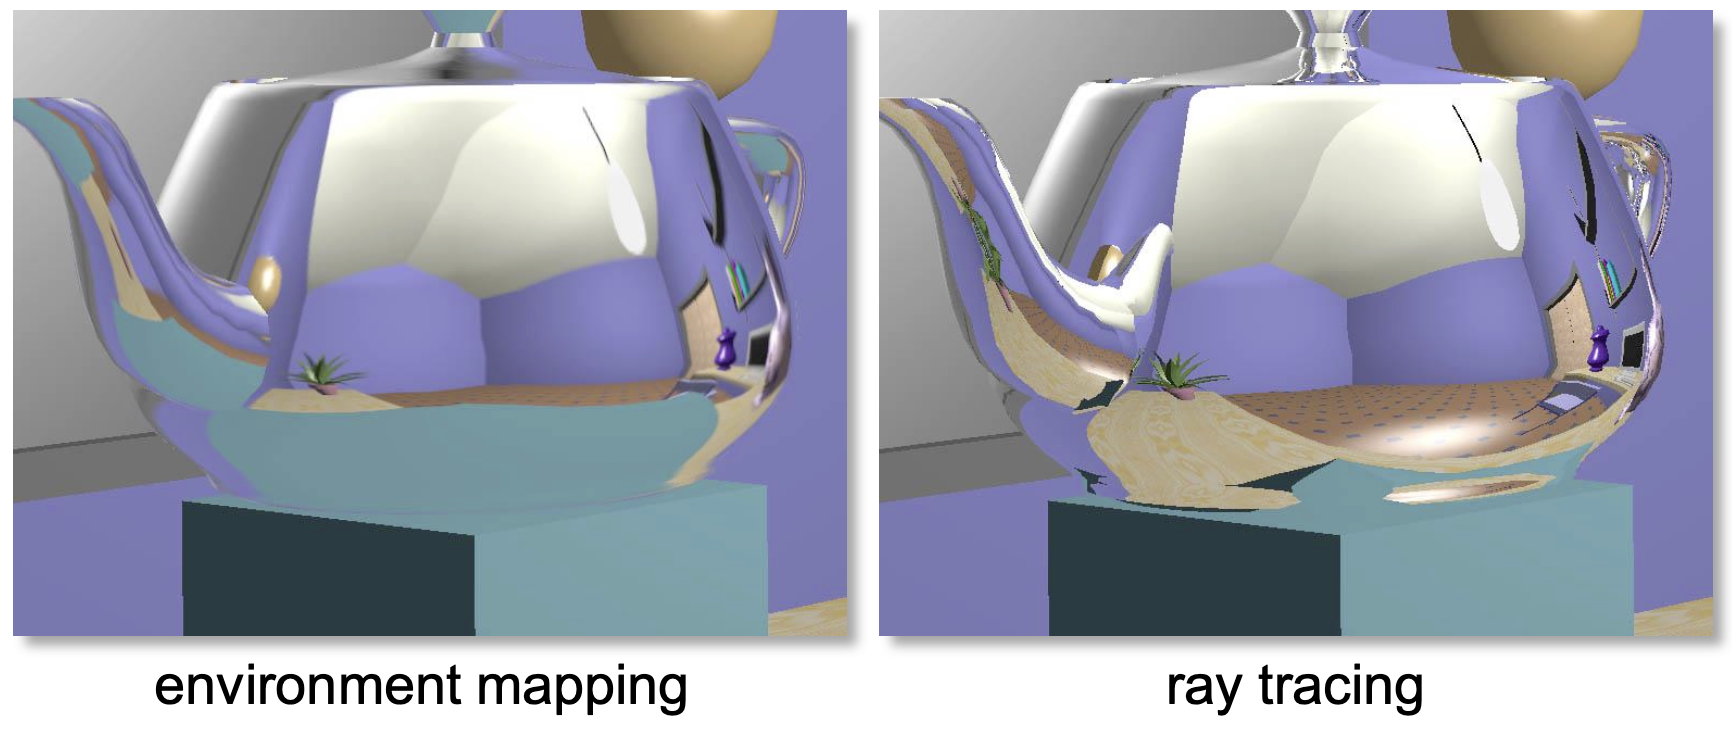
\includegraphics[width=\columnwidth]{L8/environment_mapping}
      \end{center}
      \begin{itemize}[leftmargin=*]
        \item Shortcut for rendering shiny objects
        \item Used in Lab 3
        \item Geometrically correct only when the object is a point, and/or the surrounding is infinitely far away
        \item Cannot produce self reflection
      \end{itemize}
      \paragraph{Implementation}
        \begin{itemize}[leftmargin=*]
          \item Image of surrounding is first captured (from the position where the object is to be placed) and stored in a texture map
          \item When rendering the object, the reflected eye ray is used to reference the texture map
        \end{itemize}
    \subsubsection*{Cube map}
      \begin{center}
        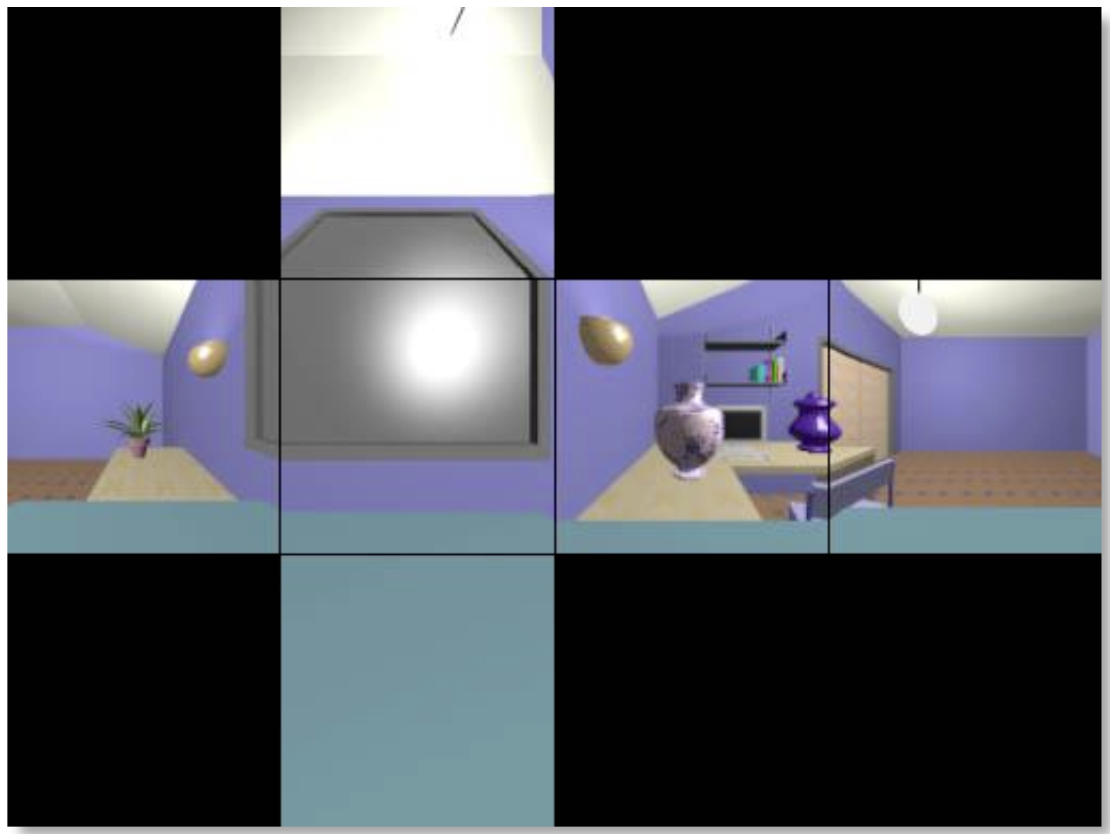
\includegraphics[width=0.8\columnwidth]{L8/cube_map}
      \end{center}
      \begin{itemize}[leftmargin=*]
        \item Image of the environment can be stored in a cube map
        \item Consists of 6 separate images pieced together, situated in the $+x, -x, +y, -y, +z, -z$ directions
      \end{itemize}
    \subsubsection*{Bump mapping}
      \begin{center}
        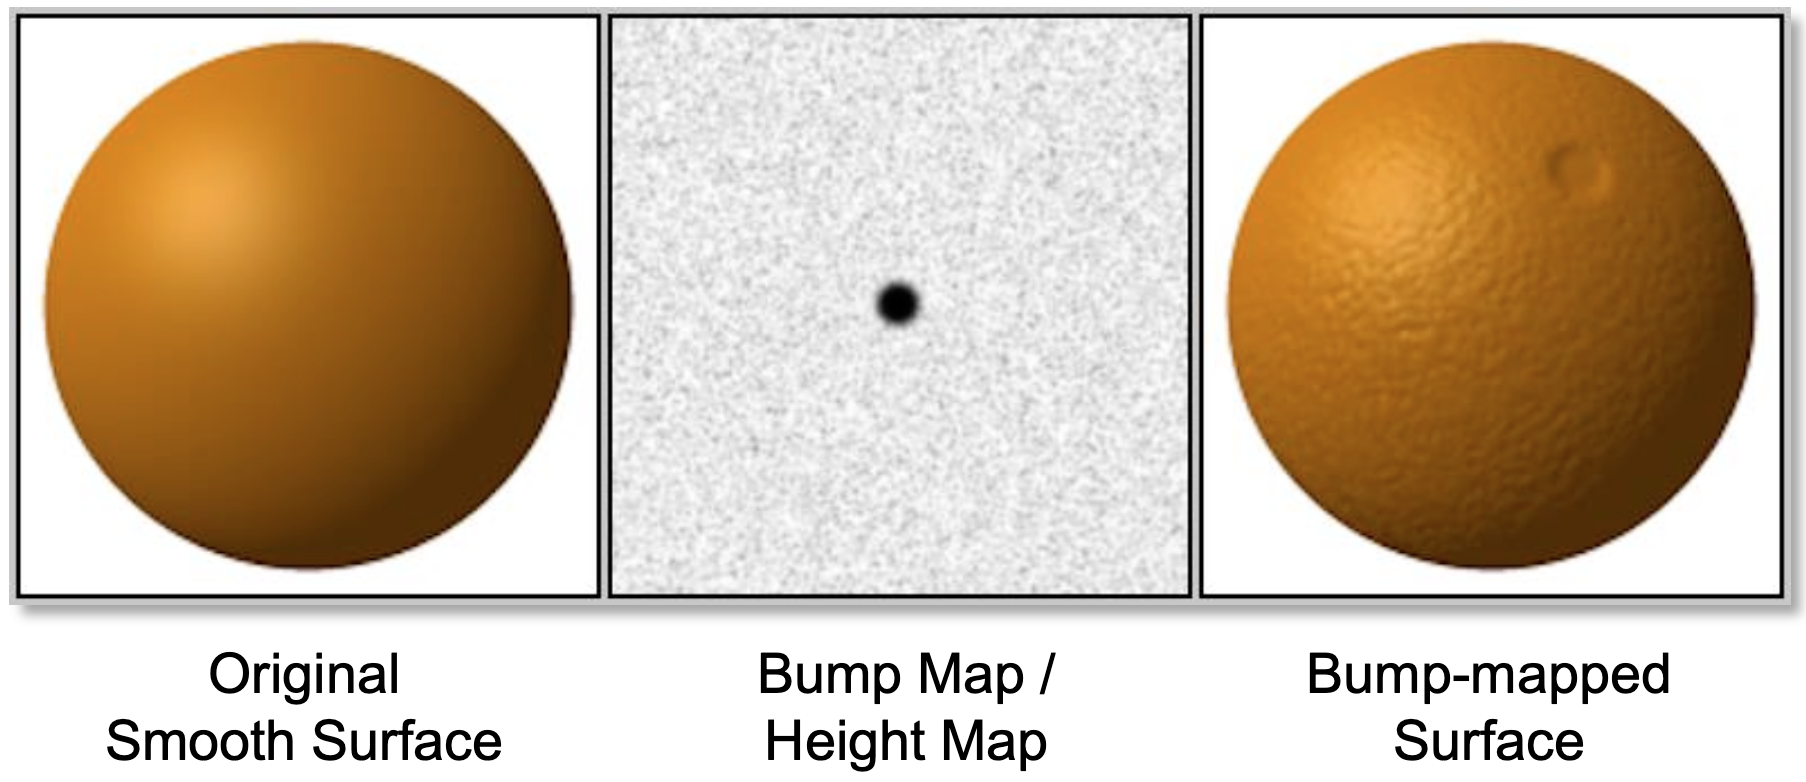
\includegraphics[width=\columnwidth]{L8/bump_mapping}
      \end{center}
      \begin{itemize}[leftmargin=*]
        \item Simulates small complex geometric features on surfaces without needing to model them
        \item Height field is used to perturb the surface normals, and the perturbed normals are used in light reflection computation
        \item Bumps facing you directly look realistic, but bumps near the silhouette will look flat
      \end{itemize}
      \begin{center}
        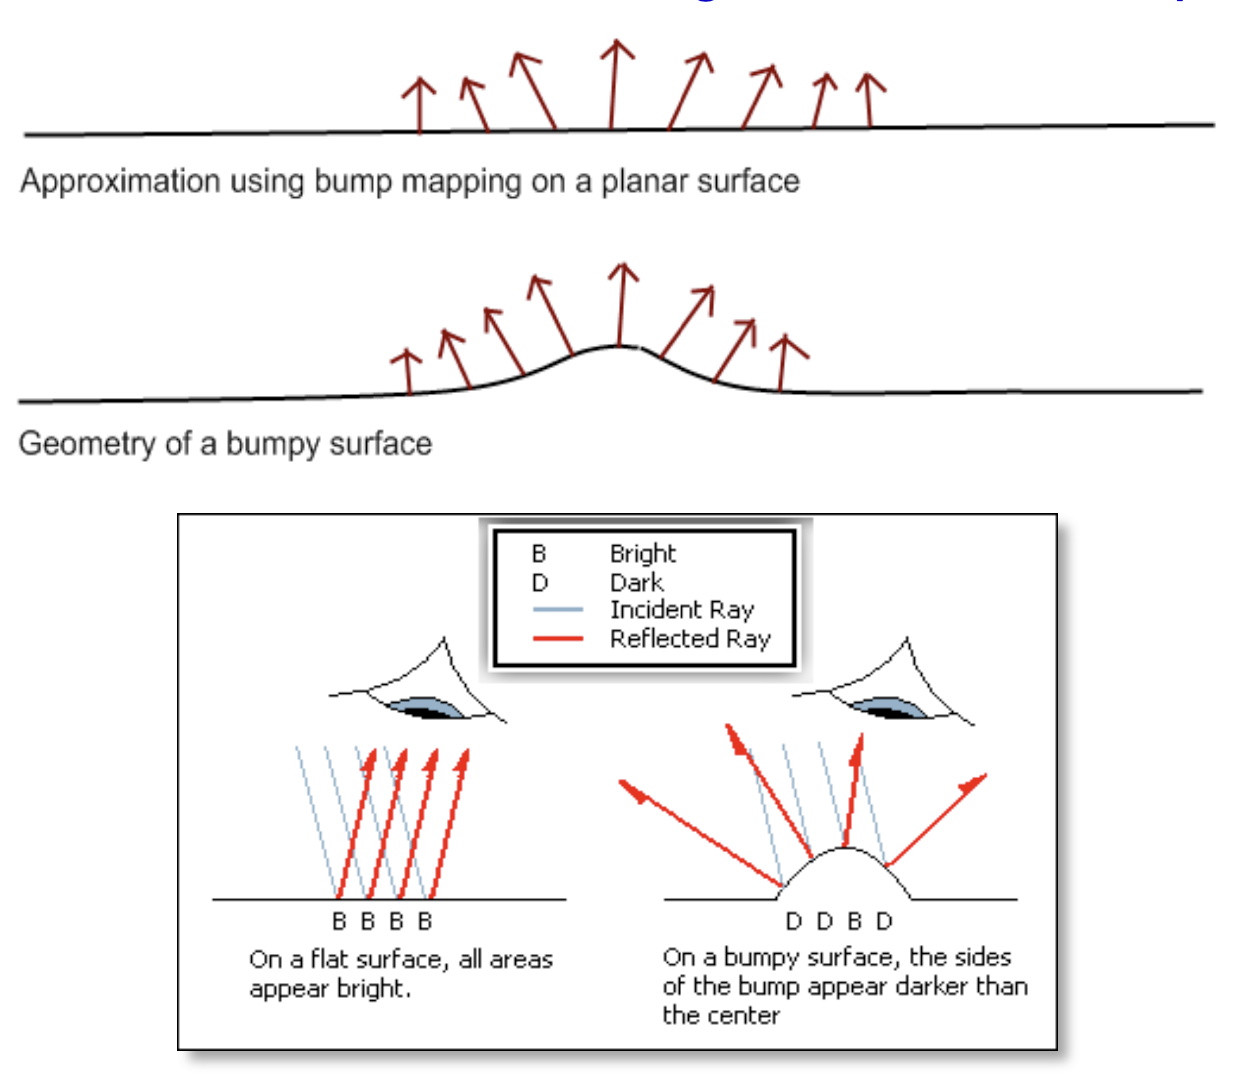
\includegraphics[width=\columnwidth]{L8/perturb}
      \end{center}
    \subsubsection*{Billboarding}
      \begin{center}
        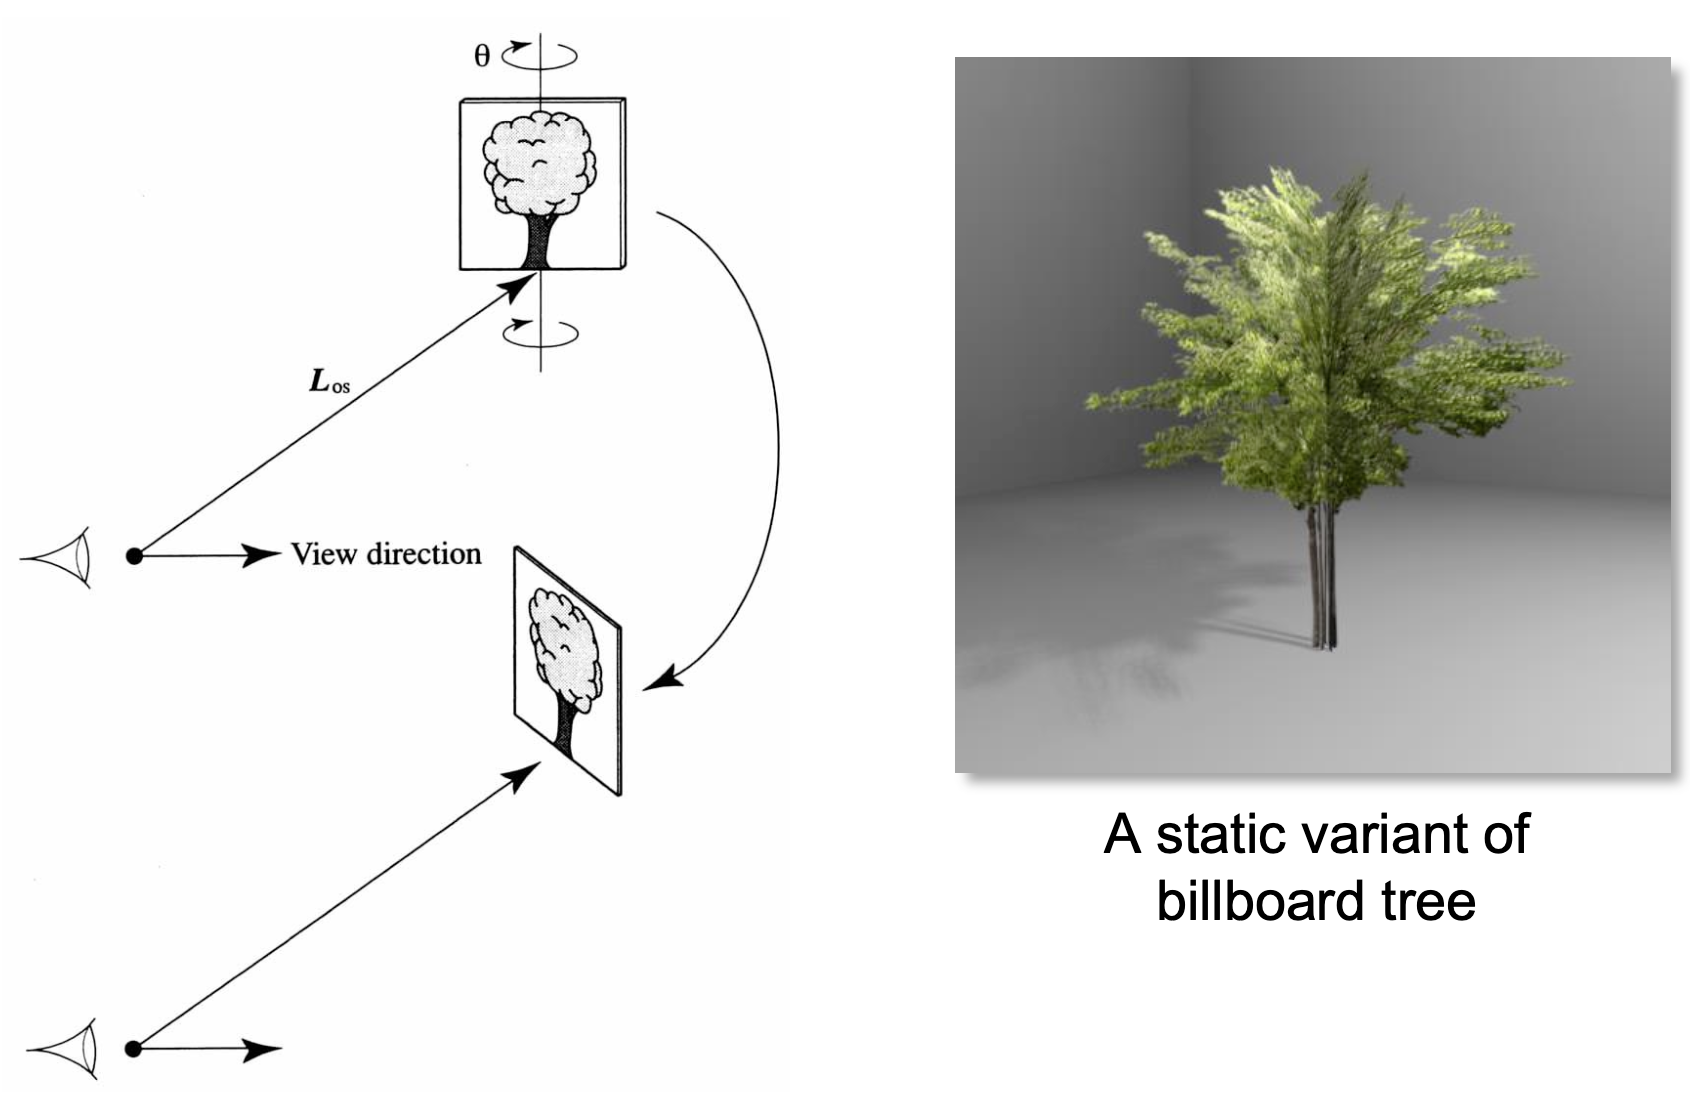
\includegraphics[width=\columnwidth]{L8/billboarding}
      \end{center}
      \begin{itemize}[leftmargin=*]
        \item Image is dynamically rotated so it is always facing you (normal is parallel to view direction)
      \end{itemize}
    \subsubsection*{3D texture mapping}
      \begin{itemize}[leftmargin=*]
        \item Does not have the downsides of 2D texture mapping
          \begin{itemize}[leftmargin=*]
            \item Texture distortions
            \item Hard to parameterize non-trivial surface topology
          \end{itemize}
        \item 3D texture is defined everywhere in 3D space (usually procedurally generated to save memory)
        \item 3D function is evaluated at 3D surface point to obtain texture value
        \item Analogous to sculpting or carving an object out of a block of material
      \end{itemize}
  \subsection*{Texture mapping in OpenGL}
    \begin{itemize}[leftmargin=*]
      \item Occurs during fragment processing stage, after a color assigned to the fragment
      \item The fragment color can be either
        \begin{itemize}[leftmargin=*]
          \item Modified by texture access (using texture corodinates), or
          \item Combined with the texture color by texture application
        \end{itemize}
      \item For implementation, refer to external slides
    \end{itemize}
\section*{Ray tracing}
  \subsection*{Ray casting}
    \begin{lstlisting}
For each pixel
    Construct a ray from the eye
    For each object in the scene
        Find intersection with the ray
        Keep if closest
    Shade // depending on light and normal vector (e.g. Phong reflection model)
    \end{lstlisting}
    \begin{itemize}[leftmargin=*]
      \item Achieves hidden surface removal naturally
    \end{itemize}
    \subsubsection*{Rasterization vs ray casting}
      \begin{itemize}[leftmargin=*]
        \item Rasterization: given a primitive in 3D space, determine which pixels are covered by the primitive
          \begin{itemize}[leftmargin=*]
            \item Hard to produce global illumination
          \end{itemize}
        \item Ray casting: given a pixel, determine which primitive covers it
          \begin{itemize}[leftmargin=*]
            \item Entire scene data must be available when computing each pixel
          \end{itemize}
      \end{itemize}
  \subsection*{Ray tracing} \noindent
    From the closest intersection point, secondary rays are shot out
    \begin{itemize}[leftmargin=*]
      \item Reflection ray
      \item Refraction ray
      \item Shadow rays (to each light source)
    \end{itemize}
\section*{\normalsize Whitted ray tracing}
  \begin{itemize}[leftmargin=*]
    \item Also called recursive ray tracing
  \end{itemize}
  \subsection*{Equation}
    \begin{center}
      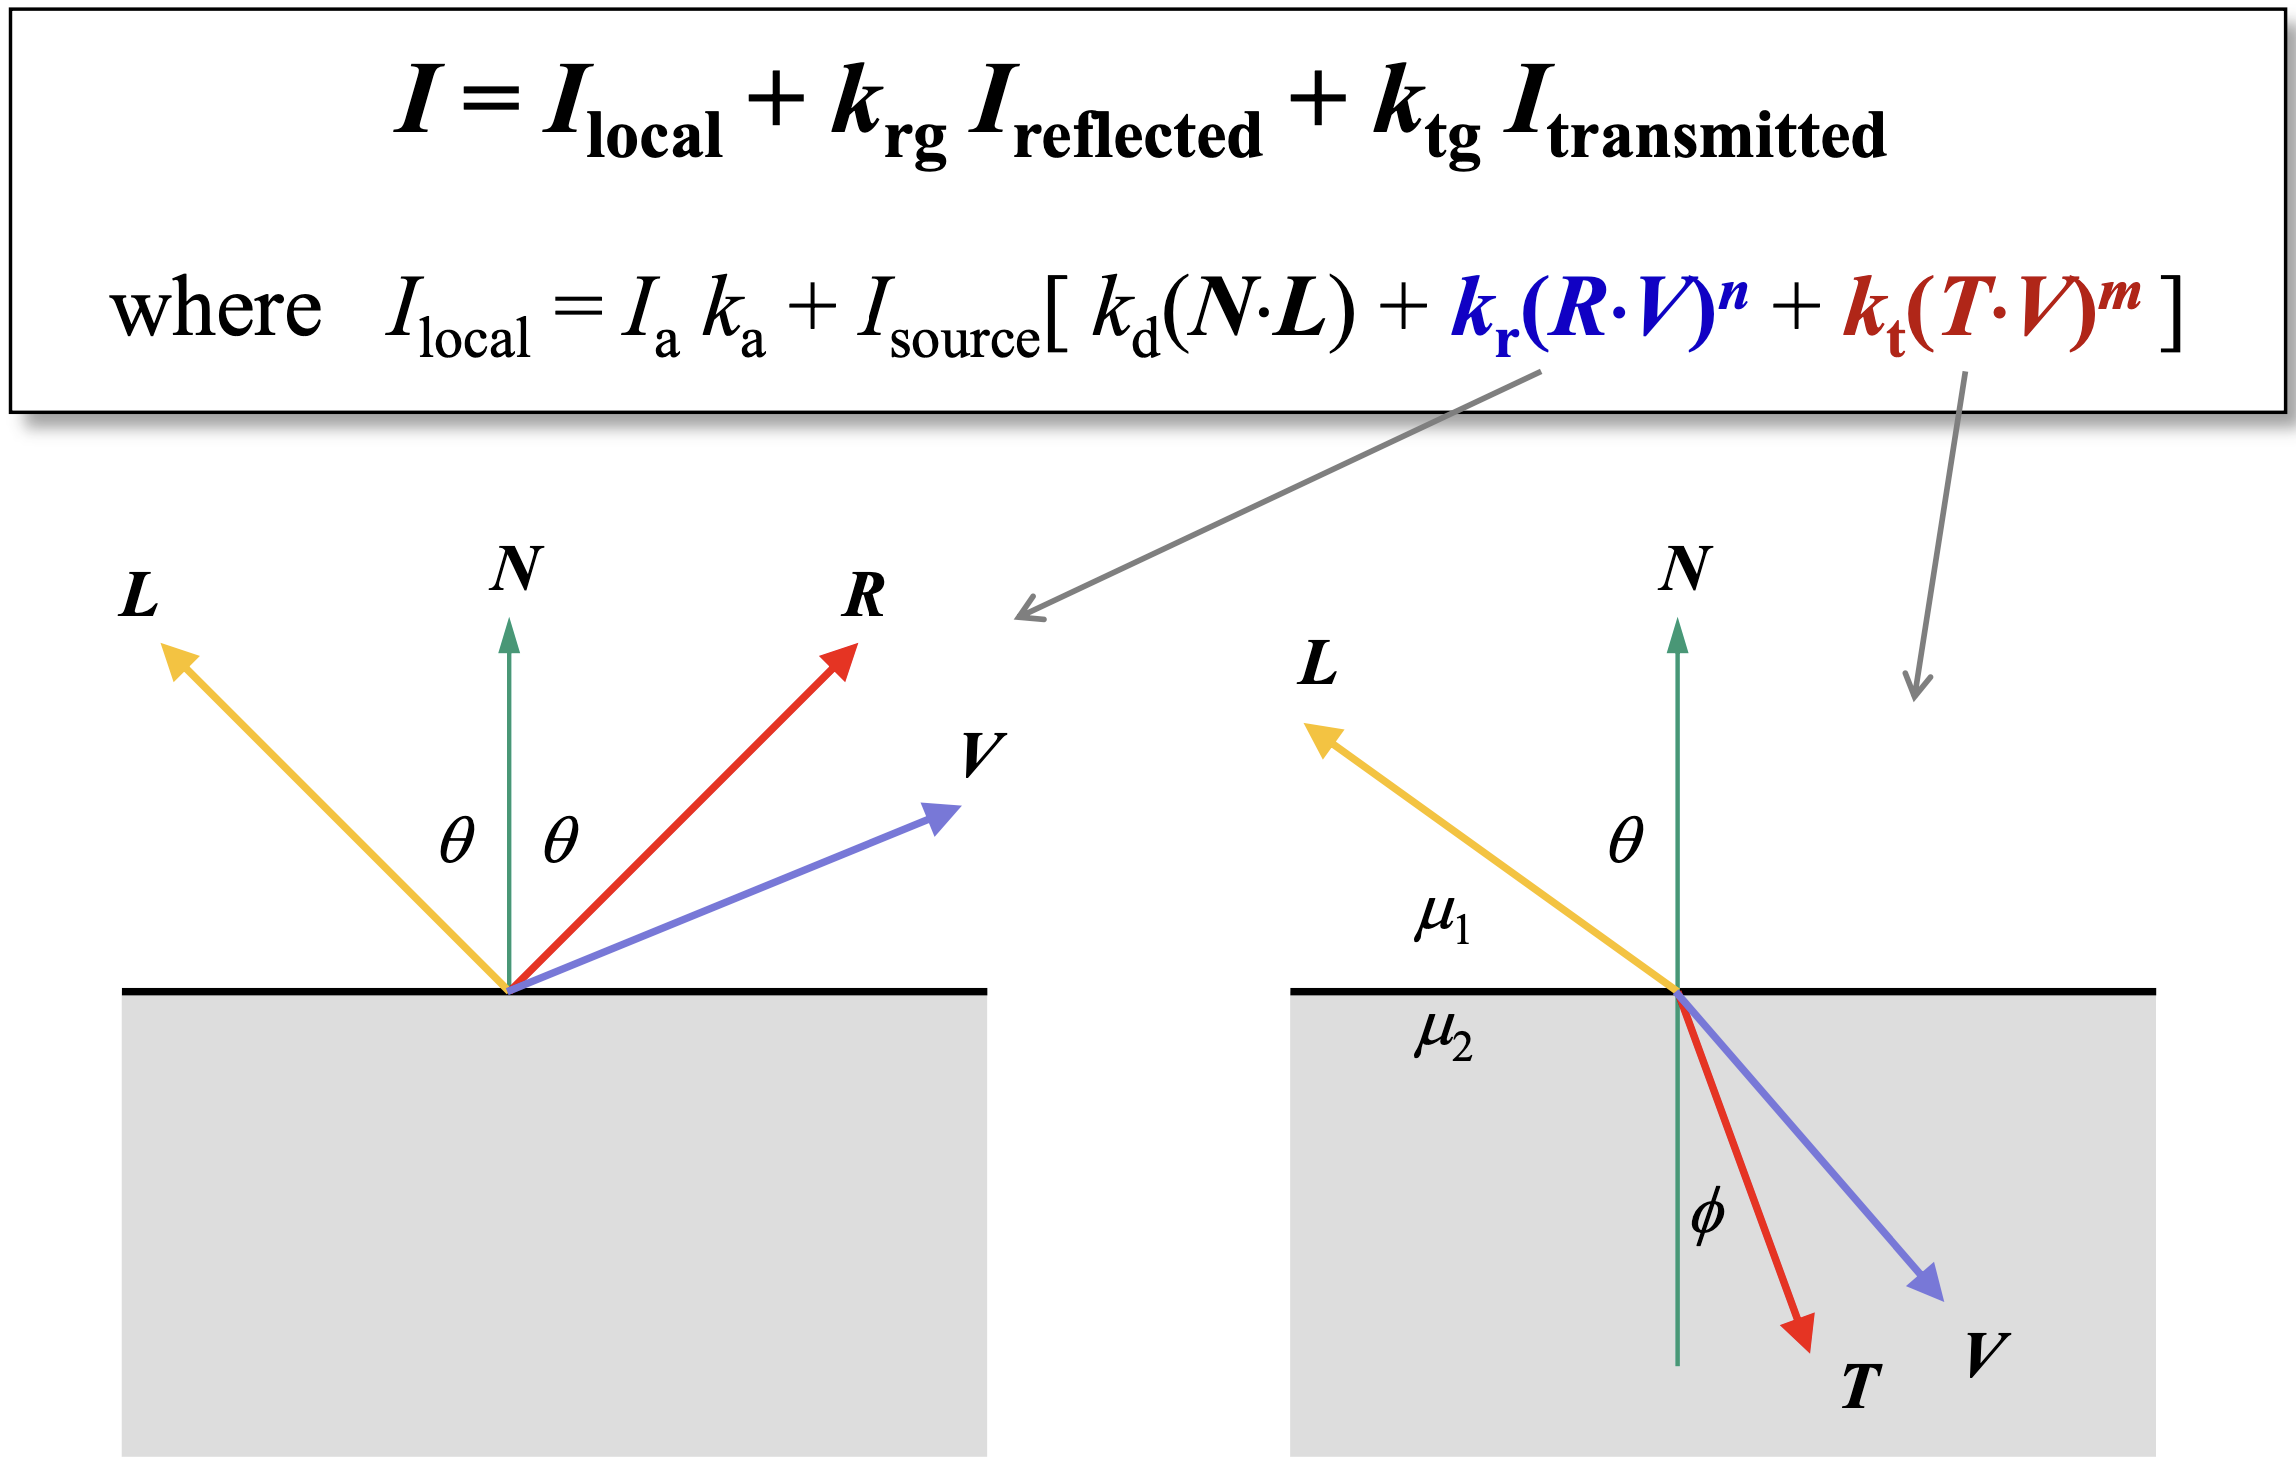
\includegraphics[width=\columnwidth]{L9/ray_tracing_equation}
    \end{center}
    \begin{itemize}[leftmargin=*]
      \item Similar to the Phong illumination equation, except specular computation is split into the reflected part and the transmitted/refracted part
      \item $k_r (R \cdot V)^n$ refers to the specular reflection
      \item $k_t (T \cdot V)^m$ refers to the transmitted/refracted specularity
      \item $k_{rg}$ stands for global reflection, because the effect is a global effect, coming from another object
      \item Similarly, $k_{tg}$ stands for global transmission
      \item If surface is opaque, ignore refracted specularity term
    \end{itemize}
    \subsubsection*{Computing reflection/refraction ray}
      \begin{center}
        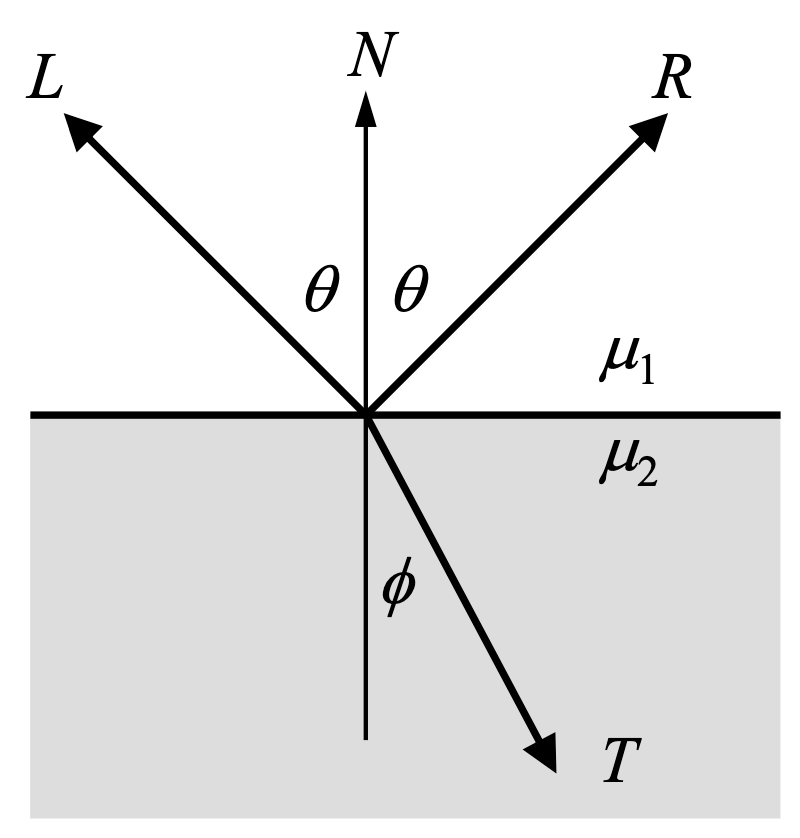
\includegraphics[width=0.7\columnwidth]{L9/ray_computation}
      \end{center}
      \begin{itemize}[leftmargin=*]
        \item Assume all vectors are unit vectors
      \end{itemize}
      \paragraph{Reflection ray}
        Like in the Phong illumination model, $R = 2 (N \cdot L) N - L$
      \paragraph{Refraction ray}
        \begin{itemize}[leftmargin=*]
          \item Snell's law: $\mu_1 \sin\theta = \mu_2 \sin \phi$
          \item Define $\mu = \mu_1 / \mu_2$, then
        \end{itemize}
        \begin{align*}
          T &= -\mu L + \Big(\mu \cos \theta - \sqrt{1 - \mu^2 ( 1 - \cos^2\theta )} \Big) N \\
          &= -\mu L \; + \\
          &\Big(\mu (N \cdot L) - \sqrt{1 - \mu^2 ( 1 - (N \cdot L)^2 )} \Big) N
        \end{align*}
    \subsubsection*{Shadow rays}
      \begin{itemize}[leftmargin=*]
        \item Also called light rays or shadow feelers
        \item From each surface intersection point, a shadow ray is shot towards each light source, to determine if there is any occlusion \uline{between} light source and surface point
        \item If occluder is opaque, then the object is occluded.
          \begin{gather*}
            I_{Phong} = \; I_a k_a + k_{shadow} I_{source} \Big[ \\
            k_d (N \cdot L) + k_r (R \cdot V)^n + k_t (T \cdot V)^m \Big]
          \end{gather*}
        \item If translucent, then
          \begin{itemize}[leftmargin=*]
            \item Light is attenuated (reduced) by the $k_{tg}$ of the occluder
            \item However, it is also affected by the distance the light travels through the occluder (i.e. the size of the occluder), but this is not accounted for
            \item Additionally, refraction of light ray from light source is ignored
            \item Both are physically incorrect, but this approach is taken to save on computation, as it is expensive to compute the realistic scenario
          \end{itemize}
      \end{itemize}
  \subsection*{Describing a scene}
    \begin{itemize}[leftmargin=*]
      \item Camera view and image resolution
        \begin{itemize}[leftmargin=*]
          \item Camera position, orientation
          \item Field of view
          \item Image resolution
        \end{itemize}
      \item Point light sources
        \begin{itemize}[leftmargin=*]
          \item Position
          \item Brightness, color
          \item Global ambient light
        \end{itemize}
      \item Object materials
        \begin{itemize}[leftmargin=*]
          \item $k_{rg}, k_{tg}, k_a, k_d, k_r, k_t$ (each is a RGB vector)
          \item $n, m$
          \item Refractive index $\mu$ if $k_{tg} \neq 0$ or $k_{rg} \neq 0$ (can use different $\mu$ for R, G, B)
        \end{itemize}
      \item Objects
    \end{itemize}
  \subsection*{Recursive ray tracing}
    \begin{center}
      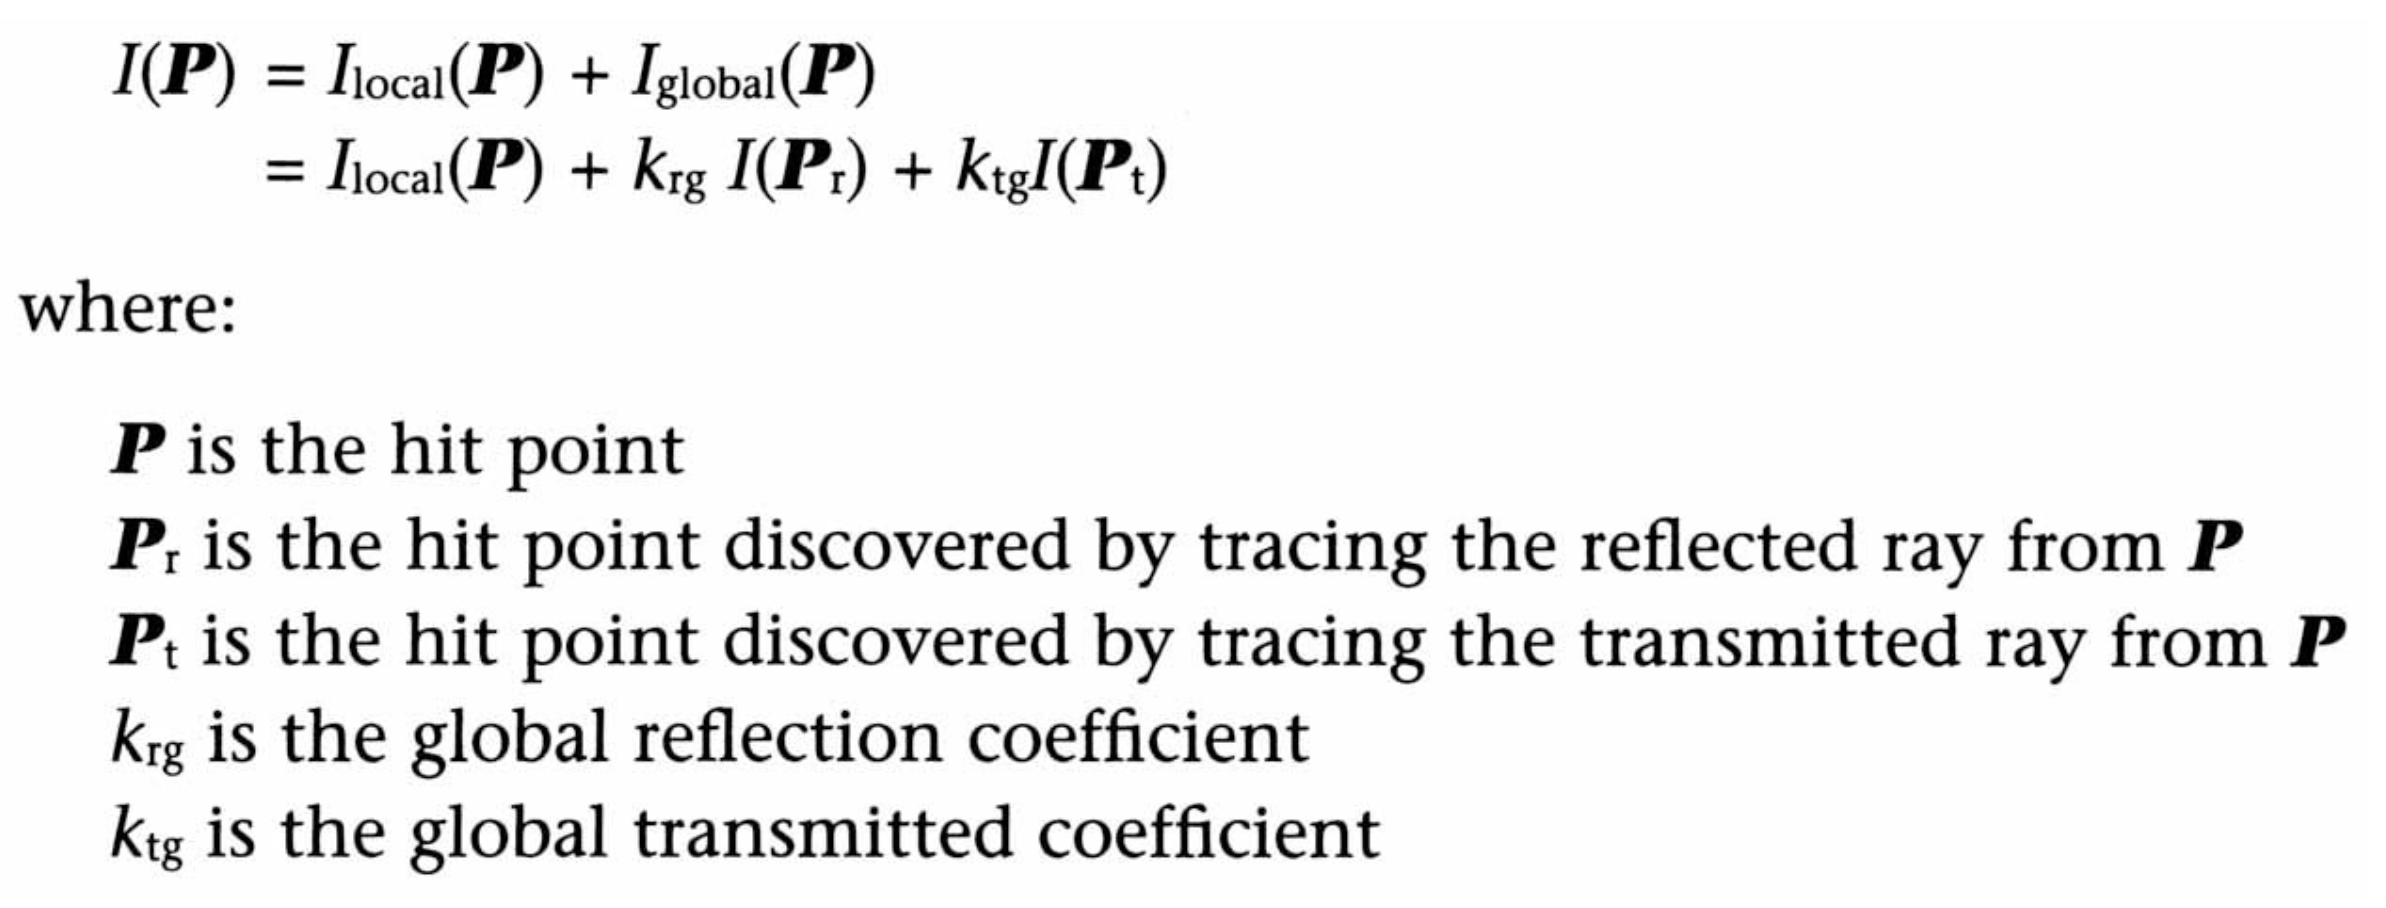
\includegraphics[width=\columnwidth]{L9/recursive}
    \end{center}
    For each reflection/refraction ray spawned, we can trace it just like tracing the original ray
    \subsubsection*{When to stop recursion}
      \begin{itemize}[leftmargin=*]
        \item When surface is totally diffuse (and opaque)
        \item When reflected/refracted ray hits nothing
        \item When recursion depth threshold is reached
        \item When the contribution of the reflected/refracted ray to the color is too small (less than a threshold)
          \begin{itemize}[leftmargin=*]
            \item Product of reflection/transmission constants that represents the path of the light ray
            \item e.g. refracted twice, reflected once:
          \end{itemize}
      \end{itemize}
      \[ k_{tg1} \times k_{tg2} \times k_{rg3} \]
      \[ (k_{rg1} \vert k_{tg1}) \times (k_{rg(n-1)} \vert k_{tg(n-1)}) < \text{threshold} \]
  \subsection*{Limitations}
    \paragraph{Hard shadows}
      \begin{itemize}[leftmargin=*]
        \item A point is either in a shadow or not
        \item Light sources assumed to be point light sources
      \end{itemize}
    \paragraph{Aliasing} (also known as jaggies)
      \\\\
      The following picture shows jaggies and a hard shadow
      \begin{center}
        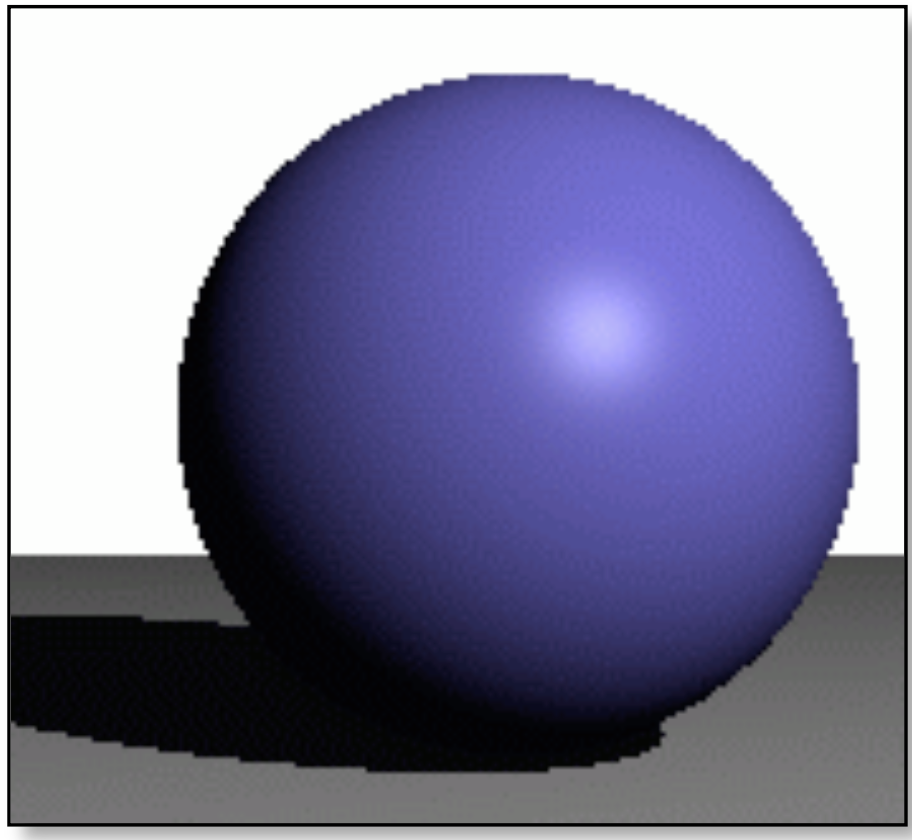
\includegraphics[width=0.7\columnwidth]{L9/limitations/jaggies}
      \end{center}
    \paragraph{Inconsistency between highlights and reflections}
      \begin{center}
        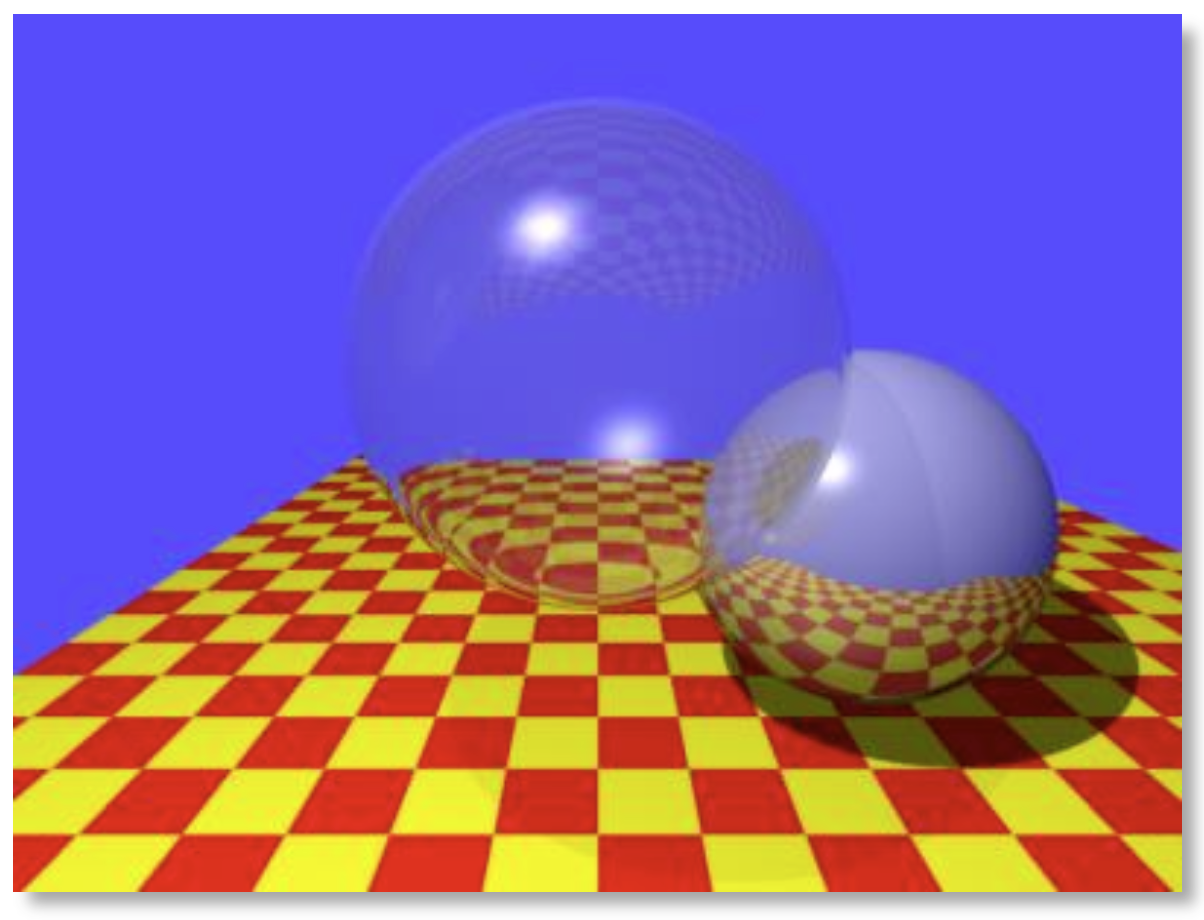
\includegraphics[width=0.7\columnwidth]{L9/limitations/inconsistency}
      \end{center}
      \begin{itemize}[leftmargin=*]
        \item We have sharp reflections (of the scene), but blurred highlights
        \item This is because they were computed via different methods: reflection is computed via reflection rays, while highlights are computed via Phong illumination model
      \end{itemize}
    \paragraph{Simulates only partial global illumination}
      \begin{center}
        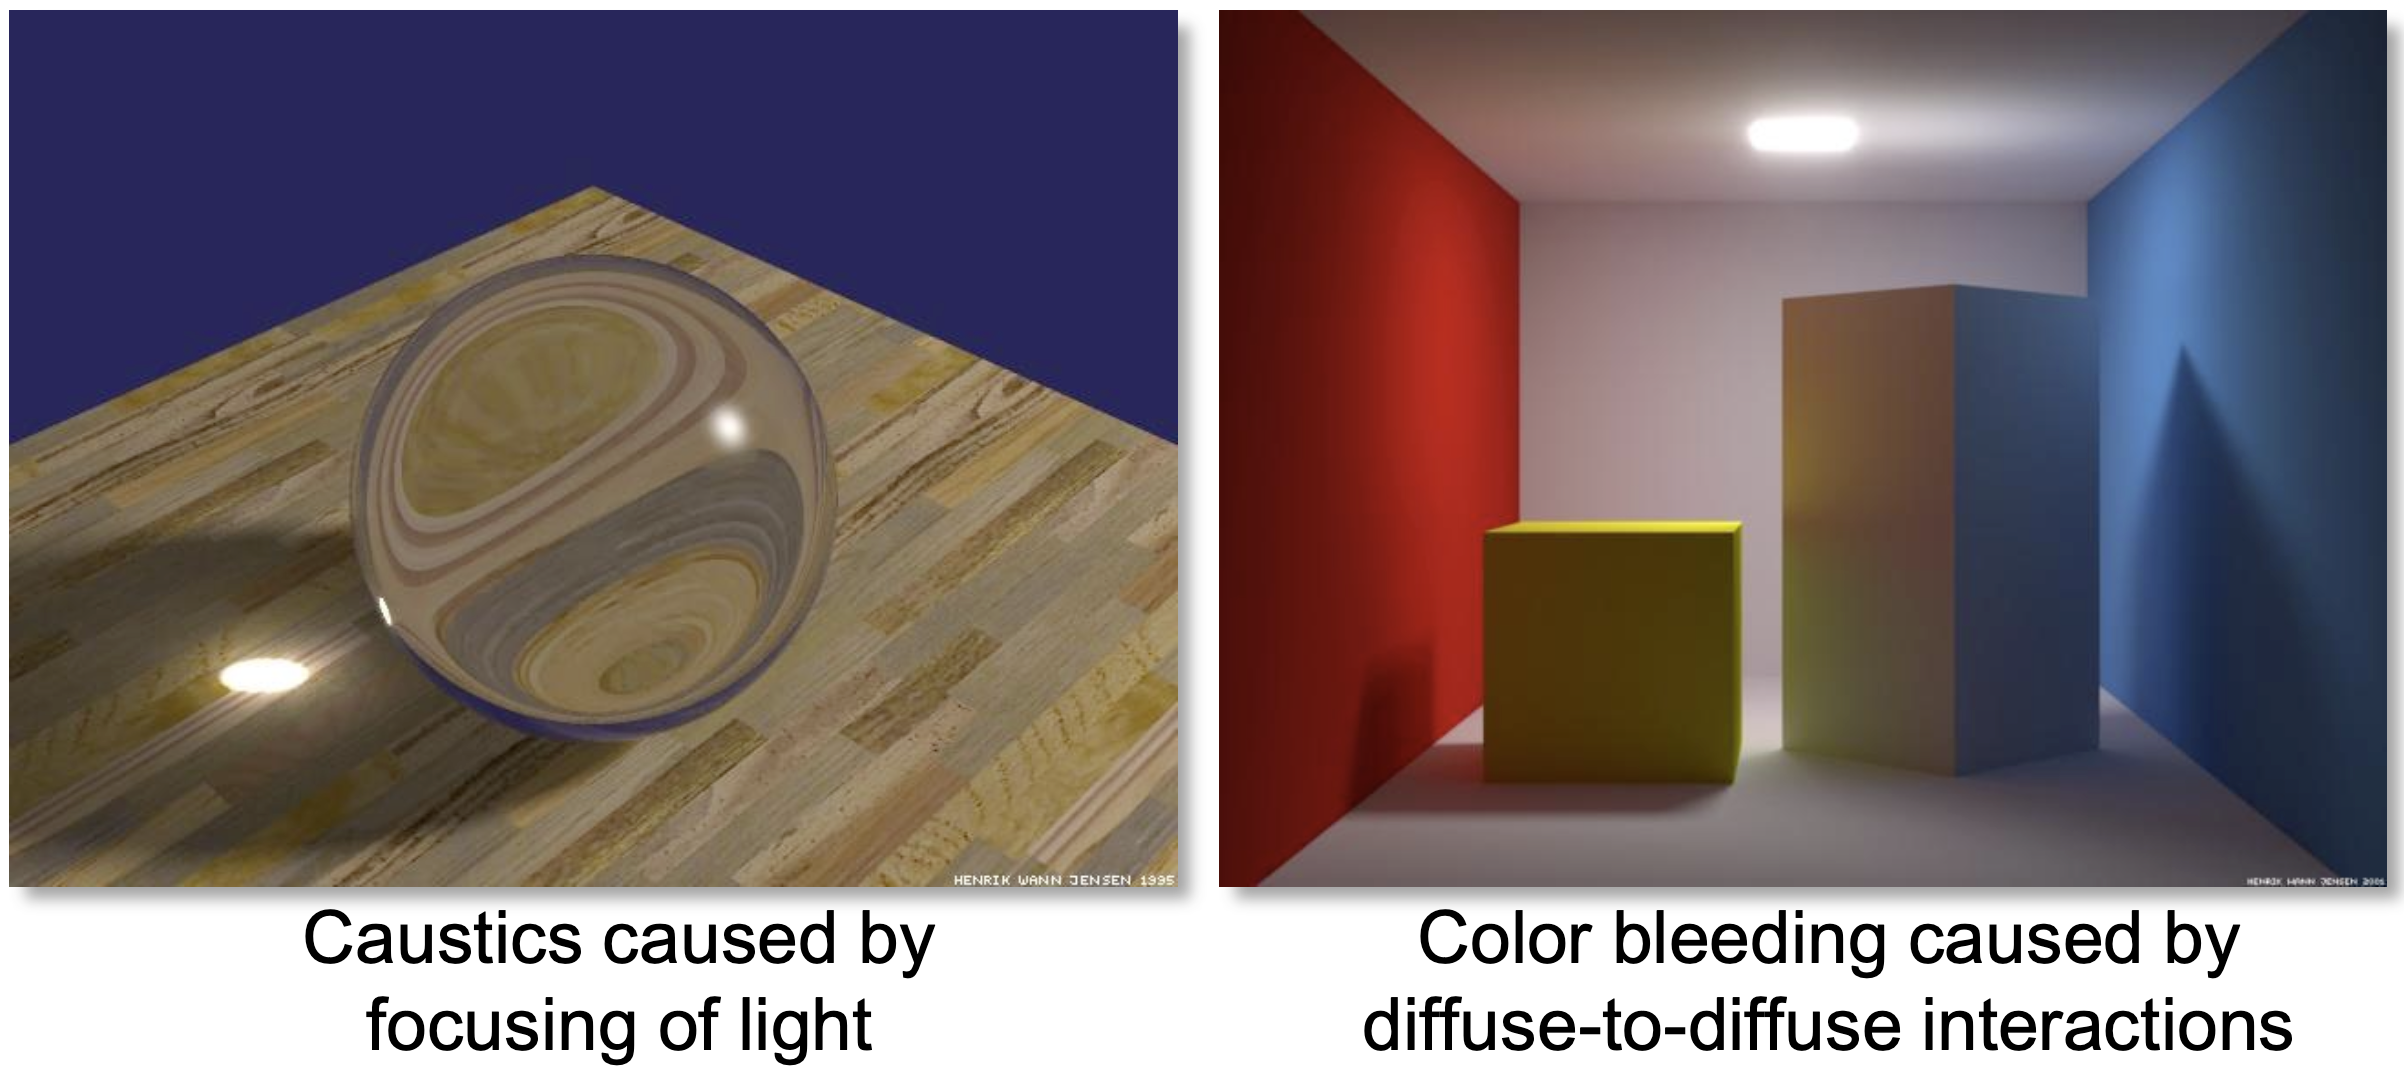
\includegraphics[width=\columnwidth]{L9/limitations/global_illumination}
      \end{center}
      \begin{itemize}[leftmargin=*]
        \item Cannot simulate caustics
        \item Cannot simulate color bleeding, because it does not spawn secondary rays in all directions to collect potential reflect light coming from other diffuse surfaces
      \end{itemize}
  \subsection*{Counting number of rays (T8)} \noindent
    Assume the scene is enclosed, i.e. all rays will hit some object
    \begin{itemize}[leftmargin=*]
      \item 1 primary ray
      \item 1 reflection ray per level of recursion
      \item 1 refraction ray per level of recursion (assuming there are non-opaque objects)
      \item 1 shadow ray per light source, per primary, reflection, or refraction ray
    \end{itemize}
\section*{\normalsize Computing intersections}
  \subsection*{Ray representation}
    \begin{itemize}[leftmargin=*]
      \item Using two 3D vectors (origin, direction), or
      \item Using parametric form
        \[ P(t) = \text{origin} + t \times \text{direction} \]
    \end{itemize}
  \subsection*{Plane}
    \begin{itemize}[leftmargin=*]
      \item Plane is often in implicit form
        \begin{itemize}[leftmargin=*]
          \item $Ax + By + Cz + D = 0$, or
          \item $N \cdot v + D = 0$, where $N = [A \; B \; C]^T$ and $v = [x \; y \; z]^T$
        \end{itemize}
    \end{itemize}
    \subsubsection*{Intersection}
      \begin{itemize}[leftmargin=*]
        \item Substitute $v = P(t)$ and solve for $t$. The intersection is at $P(t)$.
        \item If no solution for $t$, then the ray is parallel to the plane and there is no intersection
        \item Verify that the intersection is not behind the ray origin, i.e. $t_0 > 0$
      \end{itemize}
    \subsubsection*{Normal}
      \begin{itemize}[leftmargin=*]
        \item Normal is either $N$ or $-N$
      \end{itemize}
  \subsection*{Sphere}
    \begin{itemize}[leftmargin=*]
      \item Sphere (centered at origin) often in implicit form
        \begin{itemize}[leftmargin=*]
          \item $x^2 + y^2 + z^2 = r^2$, or
          \item $v \cdot v - r^2 = 0$, where $v = [x \; y \; z]^T$
        \end{itemize}
    \end{itemize}
    \subsubsection*{Intersection}
      \begin{itemize}[leftmargin=*]
        \item Let $R_o$ be the ray origin, and $R_d$ be the ray direction.
      \end{itemize}
      \begin{gather*}
        v \cdot v - r^2 = 0 \\
        (R_o + tR_d) \cdot (R_o + t R_d) - r^2 = 0 \\
        (R_d \cdot R_d) t^2 + 2 (R_d \cdot R_o) t + (R_o \cdot R_o - r^2) = 0
      \end{gather*}
      \begin{itemize}[leftmargin=*]
        \item It is a quadratic equation in the form $at^2 + bt + c = 0$
        \item Discriminant $d = b^2 - 4ac$
          \begin{itemize}[leftmargin=*]
            \item $d < 0$: no solution
            \item $d = 0$: 1 solution
            \item $d > 0$: 2 solutions
          \end{itemize}
        \item Solutions $t_\pm = \dfrac{-b \pm \sqrt{d}}{2a}$
        \item Smallest positive $t$ value is chosen as $t_0$
        \item If sphere not centered at origin, transform the ray to sphere's local coordinate frame
      \end{itemize}
    \subsubsection*{Normal}
      \begin{itemize}[leftmargin=*]
        \item Normal is $\dfrac{P(t_0)}{\lvert P(t_0) \rvert}$
      \end{itemize}
  \subsection*{Box}
    \begin{itemize}[leftmargin=*]
      \item A 3D box is defined by 3 pairs of parallel planes, where each pair is orthogonal to the other 2 pairs
      \item If it is axis-aligned, only need to specify the coordinates of the two diagonally opposite corners, as the planes can be deduced
    \end{itemize}
    \subsubsection*{Intersection}
      \begin{itemize}[leftmargin=*]
        \item In the 2D case, there are 2 intervals, which must overlap at a common region for there to be an intersection between the ray and box
      \end{itemize}
      \begin{center}
        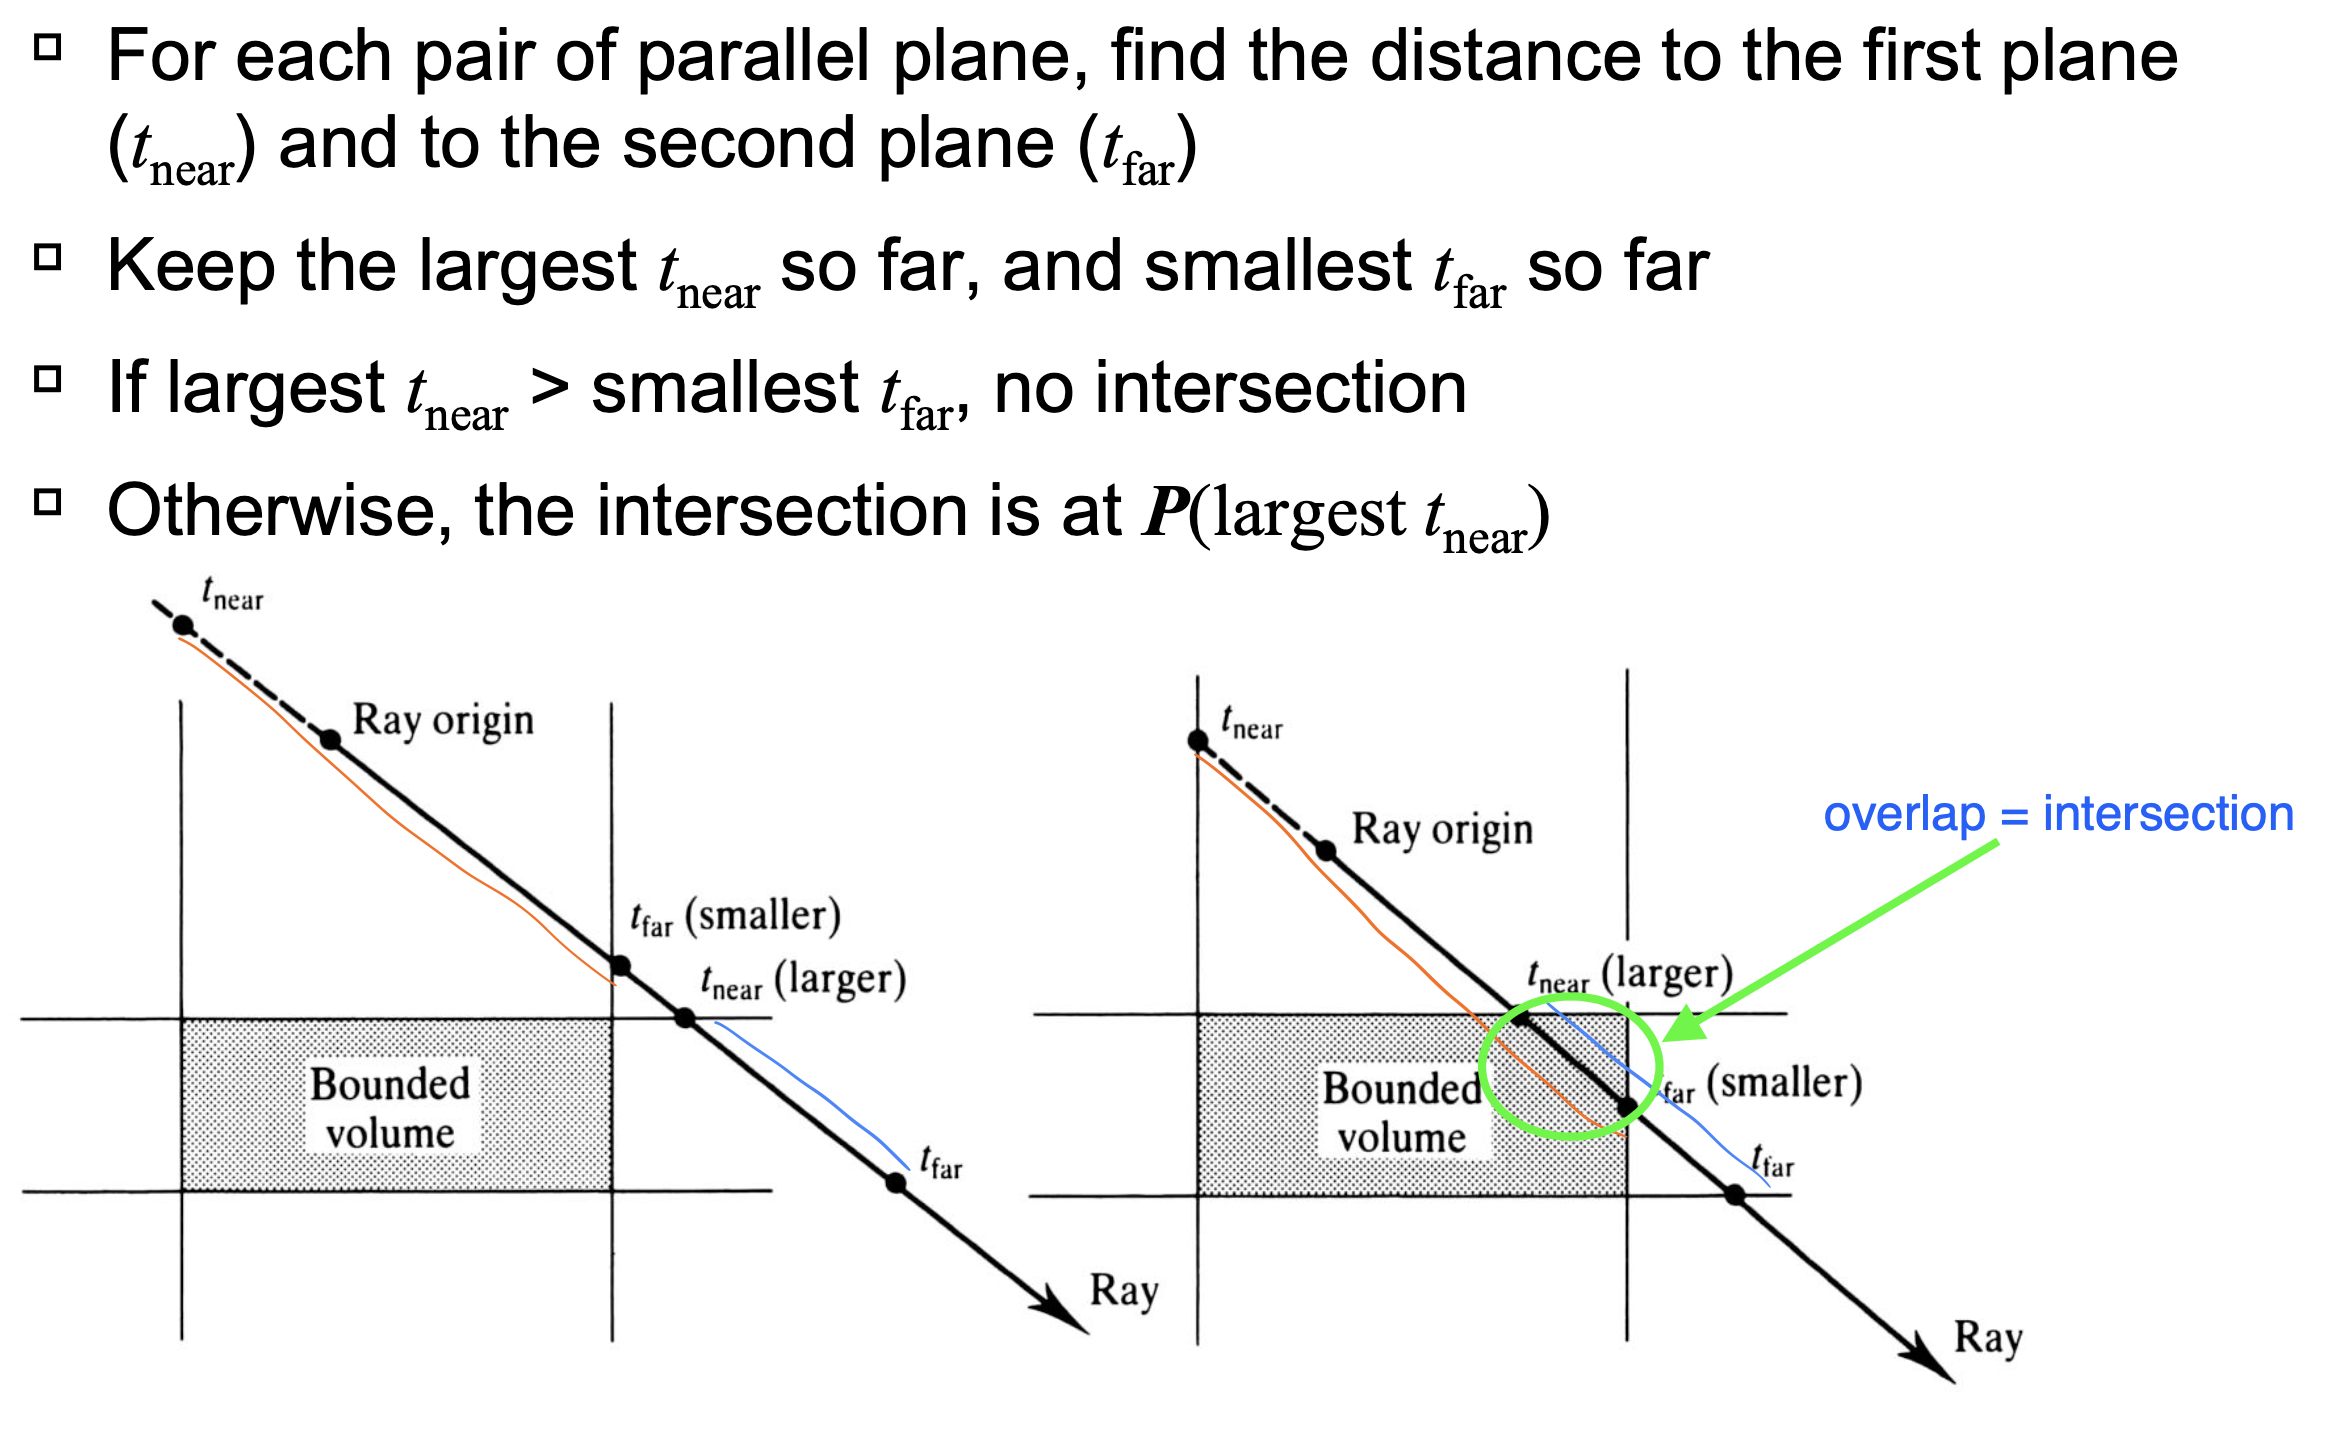
\includegraphics[width=\columnwidth]{L9/ray_box_intersection}
      \end{center}
      \begin{itemize}[leftmargin=*]
        \item In the 3D case, there are 3 intervals, which must ALL overlap at a common region for there to be an intersection between the ray and box
        \item We are not interested in knowing the exact intersection point, because boxes are usually used as bounding volumes to enclose objects, for a quick test for intersection
      \end{itemize}
    \subsubsection*{Normal} \noindent
      Can be found by considering individual planes of the box
  \subsection*{General polygon}
    \begin{itemize}[leftmargin=*]
      \item Finding intersection between a ray and a general polygon is difficult
        \begin{enumerate}[leftmargin=*]
          \item Compute ray-plane intersection (assumes polygon is planar)
          \item Determine whether intersection is within polygon (tedious for non-convex polygon)
        \end{enumerate}
        \begin{itemize}[leftmargin=*]
          \item In addition, interpolation of attributes at vertices are not well defined
        \end{itemize}
      \item Since a polygon can be decomposed into triangles, easier to find ray-triangle intersection using \uline{barycentric coordinates} method
    \end{itemize}
  \subsection*{Triangle}
    \subsubsection*{Barycentric coordinates} \noindent
      The barycentric coordinates of a point $P$ on a triangle $ABC$ is $(\alpha, \beta, \gamma)$ such that
      \[ P = \alpha A + \beta B + \gamma C \]
      where $\alpha + \beta + \gamma = 1$ and $0 \leq \alpha, \beta, \gamma \leq 1$. This can be rewritten as
      \begin{align*}
        P &= (1 - \beta - \gamma) A + \beta B + \gamma C \\
        P &= A + \beta (B-A) + \gamma (C-A)
      \end{align*}
      to eliminate one variable.
    \subsubsection*{Intersection}
      \begin{itemize}[leftmargin=*]
        \item Substitute $P(t) = P$
      \end{itemize}
      \[ R_o + t R_d = A + \beta (B-A) + \gamma (C-A) \]
      \begin{itemize}[leftmargin=*]
        \item Solve for $t, \beta, \gamma$
        \item Intersection if $\beta + \gamma < 1$ and $t, \beta, \gamma > 0$
      \end{itemize}
    \subsubsection*{Solving}
      \begin{itemize}[leftmargin=*]
        \item 3 equations, 3 unknowns: $Ax = B$
        \item Define $A_i$ as the matrix $A$ with the $i$th column replaced by $B$
        \item Cramer's rule states that the solutions are
          \[ \frac{\lvert A_1 \rvert}{\lvert A \rvert}, \frac{\lvert A_2 \rvert}{\lvert A \rvert}, \frac{\lvert A_3 \rvert}{\lvert A \rvert} \]
      \end{itemize}
    \subsubsection*{Normal} \noindent
      \[ N_P = (1 - \beta - \gamma) N_A + \beta N_B + \gamma N_C \]
      (remember to normalize)
  \subsection*{Epsilon problem} \noindent
    Should not accept intersection for very small positive $t$
    \begin{itemize}[leftmargin=*]
      \item Floating point inaccuracy might cause the ray origin to be slightly below the surface of the sphere
      \item When drawing shadow ray, the object seems to occlude itself
      \item Hence the pixel is considered occluded and a black dot is drawn
    \end{itemize}
    \begin{center}
      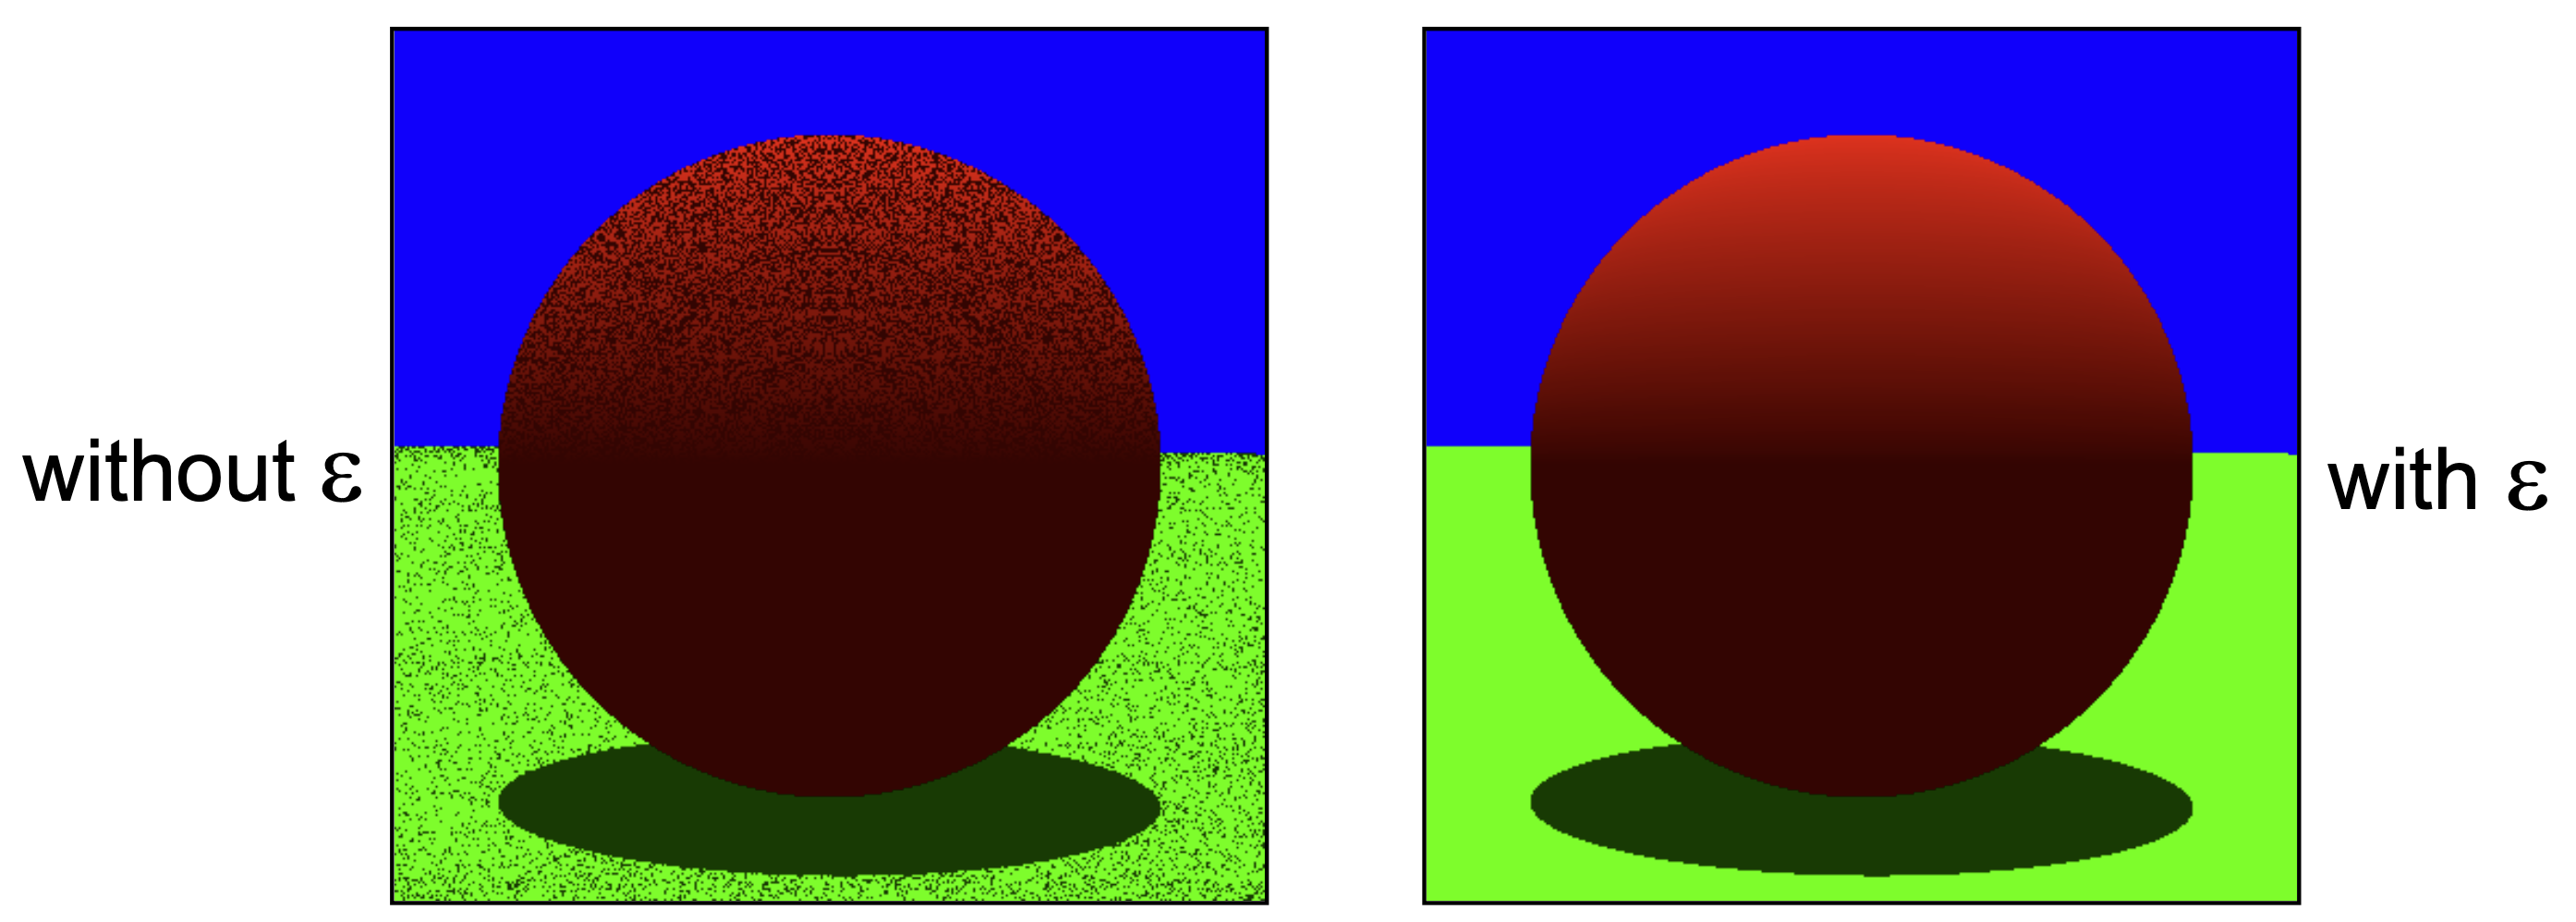
\includegraphics[width=\columnwidth]{L9/epsilon}
    \end{center}
    \subsubsection*{Solutions}
      \begin{itemize}[leftmargin=*]
        \item Method 1: Use an epsilon value $\varepsilon > 0$, and accept a intersection only if $t > \varepsilon$
        \item Method 2: When a new ray is spawned, advance the ray origin by an epsilon distance $\varepsilon$ in the ray direction
      \end{itemize}
\section*{Curves and surfaces}
  \subsection*{Misc}
    \subsubsection*{Applications}
      \begin{itemize}[leftmargin=*]
        \item Drawing vector-based smooth curves
        \item Font design, representation, and rendering
        \item Smooth animation paths
        \item Designing smooth functions
        \item 3D model design, representation, and rendering
        \item Data fitting
      \end{itemize}
    \subsubsection*{Advantages for rendering}
      \begin{itemize}[leftmargin=*]
        \item More compact representation than a set of straight line segments / set of polygons
        \item Provide scalable geometric primitives
        \item Provide smoother and more continuous primitives than straight lines / planar polygons
        \item Animation and collision detection may become simpler and faster
      \end{itemize}
    \subsubsection*{Design criteria} \noindent
      \begin{hlist}
        \item Local control of shape
        \item Smoothness and continuity
        \item Ability to evaluate derivatives
        \item Stability
        \item Ease of rendering
      \end{hlist}
  \subsection*{Representation}
    \subsubsection*{Explicit}
      \paragraph{2D curves} $y=f(x)$
        \begin{itemize}[leftmargin=*]
          \item Cannot represent vertical straight line, circle
        \end{itemize}
      \paragraph{3D curves} $y=f(x)$ and $z=g(x)$
      \paragraph{3D surfaces} $z=f(x,y)$
        \begin{itemize}[leftmargin=*]
          \item Cannot represent sphere
        \end{itemize}
    \subsubsection*{Implicit}
      \paragraph{2D curves} $f(x,y) = 0$
        \begin{itemize}[leftmargin=*]
          \item Straight line: $ax+by+c = 0$
          \item Circle: $x^2 + y^2 - r^2 = 0$
        \end{itemize}
      \paragraph{3D surfaces} $f(x,y,z) = 0$
        \begin{itemize}[leftmargin=*]
          \item Plane: $ax + by + cz + d = 0$
          \item Sphere: $x^2 + y^2 + z^2 - r^2 = 0$
        \end{itemize}
      \paragraph{3D curves}
        \begin{itemize}[leftmargin=*]
          \item Represented as the intersection of two 3D surfaces
          \item $f(x,y,z) = 0$ and $g(x,y,z) = 0$
        \end{itemize}
      \paragraph{Drawbacks} Because the equations are basically membership tests,
        \begin{itemize}[leftmargin=*]
          \item Difficult to obtain points on the curves and surfaces
          \item Rasterization is difficult (but ray tracing is easy)
        \end{itemize}
    \subsubsection*{Parametric}
      \paragraph{2D and 3D curves}
        \begin{itemize}[leftmargin=*]
          \item Each variable is expressed in terms of an independent variable $u$, the parameter
        \end{itemize}
        \[ p(u) = \begin{bmatrix} x(u) \\ y(u) \end{bmatrix} \quad p(u) = \begin{bmatrix} x(u) \\ y(u) \\ z(u) \end{bmatrix} \]
        \begin{itemize}[leftmargin=*]
          \item Tangent vector is obtained by differentiating individual components
        \end{itemize}
        \[ \dfrac{dp(u)}{du} = \begin{bmatrix} \dfrac{dx(u)}{du} & \dfrac{dy(u)}{du} & \dfrac{dz(u)}{du} \end{bmatrix}^T \]
      \paragraph{3D surfaces}
        \begin{itemize}[leftmargin=*]
          \item Uses two parameters
        \end{itemize}
        \[ p(u,v) = \begin{bmatrix} x(u,v) & y(u,v) & z(u,v) \end{bmatrix}^T \]
        \begin{itemize}[leftmargin=*]
          \item Normal vector
        \end{itemize}
        \[ n = \frac{\partial p}{\partial u} \times \frac{\partial p}{\partial v} \]
  \subsection*{\begin{varwidth}{\textwidth}
    Parametric polynomial \\ curves and surfaces
  \end{varwidth}}
    \begin{itemize}[leftmargin=*]
      \item Parametric forms are not unique
      \item Parametric forms fulfill all 5 design criteria
    \end{itemize}
    \subsubsection*{Parametric polynomial curves}
      \begin{itemize}[leftmargin=*]
        \item A parametric polynomial curve of degree $n$ or order $n+1$ is of the form
      \end{itemize}
      \begin{align*}
        p(u) &= \begin{bmatrix} x(u) \\ y(u) \\ z(u) \end{bmatrix} \\
             &= \begin{bmatrix}
               c_{x0} + c_{x1} u + c_{x2} u^2 + \cdots + c_{xn} u^n \\
               c_{y0} + c_{y1} u + c_{y2} u^2 + \cdots + c_{yn} u^n \\
               c_{z0} + c_{z1} u + c_{z2} u^2 + \cdots + c_{zn} u^n
             \end{bmatrix} \\
             &= \sum_{k=0}^n u^k c_k
      \end{align*}
      where $c_k = \begin{bmatrix} c_{xk} & c_{yk} & c_{zk} \end{bmatrix}^T$.
      \begin{itemize}[leftmargin=*]
        \item A curve \uline{segment} is defined for $u_\text{min} \leq u \leq u_\text{max}$
        \item Can assume $0 \leq u \leq 1$
      \end{itemize}
    \subsubsection*{Parametric polynomial surfaces}
      \begin{itemize}[leftmargin=*]
        \item A parametric polynomial surface is of the form
      \end{itemize}
      \[ p(u,v) = \begin{bmatrix} x(u,v) \\ y(u,v) \\ z(u,v) \end{bmatrix} = \sum_{i=0}^n \sum_{j=0}^m c_{ij} u^i v^j \]
      \begin{itemize}[leftmargin=*]
        \item $\{c_{ij}\}$ contains $3(n+1)(m+1)$ coefficients
        \item Normally, $n=m$
        \item A surface patch is defined for $0 \leq u,v \leq 1$
      \end{itemize}
    \subsubsection*{Parametric cubic polynomial curves}
      \begin{itemize}[leftmargin=*]
        \item Prefer to define long curve by joining multiple curve segments of lower degree
          \begin{itemize}[leftmargin=*]
            \item Local control of shape
            \item Stability
          \end{itemize}
        \item In particular, degree 3 / cubic parametric polynomial curve segments are preferred
        \item Can be written as
      \end{itemize}
      \[ p(u) = c_0 + c_1 u + c_2 u^2 + c_3 u^3 = \sum_{k=0}^3 u^k c_k = u^T c \]
      where
      \begin{align*}
        c &= [c_0 \; c_1 \; c_2 \; c_3]^T \\
        u &= [1 \; u \; u^2 \; u^3]^T \\
        c_k &= [c_{xk} \; c_{yk} \; c_{zk}]^T
      \end{align*}
    \subsubsection*{Specifying curve segments}
      \begin{itemize}[leftmargin=*]
        \item In practice, we don't want to specify a curve segment by directly providing the coefficients of $p(u)$
        \item We prefer to provide geometric data that can be used to derive the values of the coefficients of $p(u)$
        \item Like using control points (Bezier curves) or data points (cubic interpolating curves)
      \end{itemize}
\section*{\normalsize Cubic interpolating curves}
  \subsection*{Definition}
    \begin{itemize}[leftmargin=*]
      \item Given control points $p_0, p_1, p_2, p_3$
      \item $p(u) = c_0 + c_1 u + c_2 u^2 + c_3 u^3$ passes through all control points
      \item $p(0) = p_0$, $ p \left( \frac{1}{3} \right) = p_1$, $ p \left( \frac{2}{3} \right) = p_2$, $ p(1) = p_3$
    \end{itemize}
  \subsection*{Solving for $c$}
    \begin{itemize}[leftmargin=*]
      \item From the properties above,
    \end{itemize}
    \vspace{-0.3cm}
    \begin{align*}
      p_0 &= p(0) = c_0 \\
      p_1 &= p \left( \frac{1}{3} \right) = c_0 + \frac{1}{3} c_1 + \left( \frac{1}{3} \right)^2 c_2 + \left( \frac{1}{3} \right)^3 c_3 \\
      p_2 &= p \left( \frac{2}{3} \right) = c_0 + \frac{2}{3} c_1 + \left( \frac{2}{3} \right)^2 c_2 + \left( \frac{2}{3} \right)^3 c_3 \\
      p_3 &= p(1) = c_0 + c_1 + c_2 + c_3
    \end{align*}
    \begin{itemize}[leftmargin=*]
      \item We can also write in matrix form as $p = Ac$, where
    \end{itemize}
    \[
      p = \begin{bmatrix} p_0 \\ p_1 \\ p_2 \\ p_3 \end{bmatrix} \quad
      A = \begin{bmatrix}
        1 & 0 & 0 & 0 \\
        1 & \frac{1}{3} & \left( \frac{1}{3} \right)^2 & \left( \frac{1}{3} \right)^3 \\
        1 & \frac{2}{3} & \left( \frac{2}{3} \right)^2 & \left( \frac{2}{3} \right)^3 \\
        1 & 1 & 1 & 1
      \end{bmatrix}
    \]
    \begin{itemize}[leftmargin=*]
      \item We can solve for $c$ by performing matrix inversion, so $c = A^{-1} p = M_I p$
      \item $A^{-1} = M_I$ is called the interpolation geometry matrix, and is the same for \uline{any} 4 control points
    \end{itemize}
    \[
      M_I = \begin{bmatrix}
        1 & 0 & 0 & 0 \\
        -5.5 & 9 & -4.5 & 1 \\
        9 & -22.5 & 18 & -4.5 \\
        -4.5 & 13.5 & -13.5 & 4.5
      \end{bmatrix}
    \]
\section*{\normalsize Bezier curves}
  \subsection*{Bezier patches vs polygon mesh}
    \begin{itemize}[leftmargin=*]
      \item Bezier patches can be subdivided appropriately according to the size of the image, obtaining high rendering quality without making unnecessary computations
      \item Polygon mesh uses a fixed number of polygons. For a small image, there could be too many polygons, wasting computation. For a large image, there could be too few polygons, resulting in low rendering quality.
    \end{itemize}
  \subsection*{Flatness of a Bezier curve}
    \begin{center}
      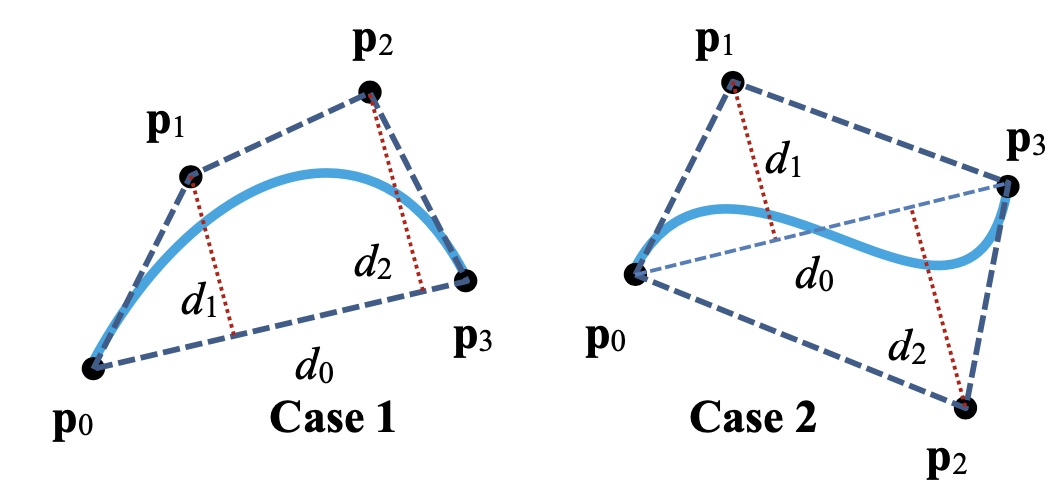
\includegraphics[width=\columnwidth]{L10/flatness}
    \end{center}
    \begin{itemize}[leftmargin=*]
      \item Let $d_1, d_2$ be the distance from $p_1, p_2$ to the line segment from $p_0$ to $p_3$. Then $d = \max(d_1, d_2)$ is a measure of flatness. The smaller the $d$, the flatter the curve
      \item Can also consider angles $\angle p_1 p_0 p_3$ and $\angle p_2 p_3 p_0$. As they get smaller, the curve gets flatter
      \item A flat Bezier curve can be drawn as a straight line segment instead
    \end{itemize}
  \subsection*{Flatness of a Bezier surface patch}
    \begin{itemize}[leftmargin=*]
      \item Define an average plane of the 4 corner control points $p_{00}, p_{03}, p_{30}, p_{33}$
      \item Find the maximum distance from the 16 control points to the average plane
    \end{itemize}
\section*{\normalsize Solving curve questions}
  \subsection*{$p(u) \rightarrow$ cubic interpolating}
    \begin{itemize}[leftmargin=*]
      \item Solve the following equations
    \end{itemize}
    \vspace{-0.5cm}
    \begin{align*}
      p_0 &= p(0) \\
      p_1 &= p(1/3) \\
      p_2 &= p(2/3) \\
      p_3 &= p(1)
    \end{align*}
  \subsection*{$p(u) \rightarrow$ bezier}
    \begin{itemize}[leftmargin=*]
      \item Obtain $p'(u)$
      \item Solve the following equations
    \end{itemize}
    \vspace{-0.5cm}
    \begin{align*}
      p_0 &= p(0) \\
      p_1 &= (p'(0) + 3p_0) / 3 \\
      p_2 &= (3p_3 - p'(1)) / 3 \\
      p_3 &= p(1)
    \end{align*}
  \subsection*{$p(u), q(u) \rightarrow$ bezier that joins with $C^1$}
    \begin{itemize}[leftmargin=*]
      \item Assume $p$ joins to $s$ joins to $q$
      \item Obtain $p'(u), q'(u)$
      \item Compute $s'(0) = p'(1)$ and $s'(1) = q'(0)$
      \item Solve the following equations
    \end{itemize}
    \vspace{-0.5cm}
    \begin{align*}
      s_0 &= p(1) \\
      s_1 &= (s'(0) + 3s_0) / 3 \\
      s_2 &= (3s_3 - s'(1)) / 3 \\
      s_3 &= q(0)
    \end{align*}
  \subsection*{bezier $\rightarrow$ split into two bezier}
    \begin{itemize}[leftmargin=*]
      \item Run De Casteljau's algorithm with approriate $t$
    \end{itemize}
  \subsection*{Joining 2 bezier curves $p$ and $q$}
    \begin{itemize}[leftmargin=*]
      \item $C^0$ continuity: $p_3 = q_0$
      \item $C^1$ continuity: we need the two tangent vectors to be the same magnitude and opposite direction - $p_3 - p_2 = q_1 - q_0$
    \end{itemize}
  \subsection*{Continuity}
    \begin{itemize}[leftmargin=*]
      \item $C^0 \iff p(1) = q(0)$
      \item $C^1 \iff p'(1) = q'(0)$
      \item $G^1 \iff p'(1) = \alpha q'(0)$ for $\alpha > 0$
    \end{itemize}
  \subsection*{Derivatives}
    \vspace{-0.5cm}
    \begin{align*}
      p(u) &= (1-u)^3 A + 3u(1-u)^2 B \\
           &+ 3u^2(1-u) C + u^3 D \\
      p'(u) &= -3(1-u)^2 A \\
            &+ \Big( 3(1-u)^2 - 6u(1-u) \Big) B \\
            &+ \Big( 6u(1-u) - 3u^2 \Big) C + 3u^2 D \\
      p'(0) &= -3A + 3B \\
      p'(1) &= -3C + 3D
    \end{align*}
\end{multicols*}
\end{document}

